%%% Неактуальный вариант из магистерской

\chapter[Полигональные системы и их деформации]
    {Полигональные системы и их деформации}


\section[Стягиваемые полигональные системы]
    {Стягиваемые полигональные системы}


\subsection{Самоподобные множества и дендриты}

\begin{definition} 
Пусть $\eS=\{S_1, S_2, \ldots, S_m\}$ --- это система (иньективных) сжимающих отображений полного метрического пространства $(X, d)$.
Непустое компактное множество $K\IN X$ называется аттрактором системы $\eS$, если $K = \bigcup \limits_{i = 1}^m S_i (K)$.
\end{definition}

Множество $K\subset X$ также называют самоподобным относительно $S$ или {\em инвариантным множеством}  системы $\eS$.
 
Система $\eS$ определяет свой оператор Хатчинсона $T$  как  $T(A) = \bigcup \limits_{i = 1}^m S_i (A)$.
Согласно теореме Хатчинсона, аттрактор $K$ -- единственный для $\eS$, и для любого компактного множества $A\IN X$ последовательность $T^n (A)$ сходится к $K$.
Мы также называем подмножество $K\IN X $ самоподобным относительно $\eS$.\\
На протяжении всей работы предполагается, что отображения $S_i\in \eS$ являются подобиями, а множество $X$ - $\mathbb{R}^2$.
Мы будем использовать комплексные обозначения для точки на плоскости, поэтому каждое подобие будет записано как $S_j(z)=q_je^{i\al_j}(z-z_j)+z_j$, где $q_j=\Lip S_j$ и $z_j=\fix(S_j)$.
Для системы $\eS$, пусть $q_{min}=\min\{q_j,j\in I\}$ и $q_{max}=\max\{q_j,j\in I\}$.\\
Здесь $I=\{1,2,...,m\}$ --- это индексное пространство, в то время как $\ia=\bigcup\limits_{n=1}^\8 I^n$ является множеством всех мультииндексов $\bj=j_1j_2...j_n$.
Длина $n$ мультииндекса $\bj=j_1...j_n$ обозначается через  $|\bj|$, а $\bi\bj$  обозначает конкатенацию соответствующих мультииндексов.
Мы говорим, что $\bi\sqsubset\bj$, если  $\bj=\bi\bl$ для некоторого $\bl\in\ia$, и если $\bi\not\sqsubset\bj$ и $\bj\not\sqsubset\bi$, где $\bi$ и $\bj$ {\em несравнимы}.\\

Для мультииндекса $\bj\in\ia$ мы пишем $S_\bj=S_{j_1j_2...j_n}=S_{j_1}S_{j_2}...S_{j_n}$ и для множества $A \subset X$ мы обозначим $S_\bj(A)$ как $A_\bj$; мы также обозначим через $G_\eS=\{S_\bj, \bj\in\ia\}$ полугруппу, порожденную системой $\eS$;\\
$I^{\8}=\{{\bf \al}=\al_1\al_2\ldots,\ \ \al_i\in I\}$ обозначает индексное пространство; и $\pi:I^{\8}\rightarrow K$ --- это {\em индексное отображение}, переводящее $\bf\al$ в точку $\bigcap\limits_{n=1}^\8 K_{\al_1\ldots\al_n}$.\\
Вместе с системой $\eS$ мы можем рассматривать её n-ную итерацию $\eS^{(n)}=\{S_\bj, \bj\in I^n\}$, оператор Хатчинсона которой равен $T^n$.

\begin{definition}
Система ${\eS}$ удовлетворяет {\em условию открытого множества} (OSC), если существует непустое открытое множество $O \IN X$ такое, что $S_i (O), \{1 \le i\le m\}$ попарно непересекаются и все содержатся в $O$.
\end{definition}

Пусть $\eC$ --- это объединение всех  $S_i(K)\cap S_j(K)$, $i,j \in I, i\neq j$.
{\em Посткритическое множество} $\eP$ системы $\eS$ --- это множество всех $\alpha\in I^{\8}$ таких, что для некоторых ${\bf j}\in I^*$, $S_ {\bf j}(\alpha)\in\eC$. 
Другими словами, $\eP= \lbrace \sigma^k(\alpha) : \alpha\in \eC,k\in \mathbb{N}\rbrace$, где отображение $\sigma^k:I^{\8}\to I^{\8}$ определяется как $\sigma^k(\al_1\al_2\ldots)=\al_{k+1}\al_{k+2}\ldots$
Система $\eS$ называется {\em посткритически конечной} (PCF) \cite{Kig}, если её посткритическое множество $\eP$ конечно. 
Таким образом, если система  $\eS$ посткирически конечна, то существует конечное множество $\eV=\pi(\eP)$ такое, что для любых несравнимых $\bi,\bj\in\ia$,  $K_\bi\cap K_\bj= S_\bi(\eV)\cap S_\bj(\eV)$.

\begin{definition}
Дендритом называется локально связный континуум, не содержащий простых замкнутых дуг.
\end{definition}

Порядок $Ord(p,X)$ точки $p$  относительно континуума $X$  в случае дендритов равен   числу связных компонент  множества $X \setminus \{p\}$. При этом точки порядка $1$ называются {\em концами} в $X$, а разбивающие точки делятся на обычные, если $Ord(p,X)=2$, и  {\em точки ветвления}, если $Ord(p,X)\ge3$.\\

Для континуума $X$ следующие свойства эквивалентны:\\
1) $X$ --- дендрит;\\
2) любые две различные точки в $X$ разделяются третьей;\\
3) всякая точка $p\in X$ --- либо конец, либо разбивающая точка;\\
4) всякий невырожденный подконтинуум в $X$ содержит несчетное множество разбивающих точек в $X$;\\
5) для любого $p \in X$ число компонент $X \setminus p$ равно $Ord(x,P)$ (если одно из них конечно);\\
6) пересечение любых двух связных подмножеств в $X$ связно;\\
7) $X$ односвязно, и для любых двух точек $x,y \in X$ существует единственная кривая $\gamma$, соединяющая $x$ и $y$.

%%%%%%%%%%%%%%%%%%%%%%%%%%%%%%%%%%%%%%%%%%%%%%%%%%%%%%%%
\subsection{Стягиваемые полигональные системы}

Пусть $P$ --- конечный гомеоморфный  диску многоугольник на плоскости и $\eV_P=\{A_1,...,A_{n_P}\}$ --- множество  его вершин. Пусть также $\Om(P,A)$ обозначает угол вершины $A$ в многоугольнике $P$.\\

Рассмотрим систему подобий $\eS = \{S_1, \ldots, S_m\}$ в ${\mathbb{R}}^2$ такую, что:\\
{\bf (D1)} для любого $i \in I$ множество $P_i = S_i (P) \subset P$;\\ 
{\bf (D2)} для любого $i \ne j, i, j \in I, P_i \bigcap P_j =  \eV_{P_i} \bigcap  \eV_{P_j}$ и $\#(\eV_{P_i} \bigcap  \eV_{P_j})<2$;\\  
{\bf (D3)} $\eV_P \subset \bigcup \limits_{i \in I} S_i (\eV_P)$;\\
{\bf (D4)} множество $\widetilde P = \bigcup \limits_{i = 1} ^m P_i$ стягиваемо.\\

\begin{definition}
Система \ $\eS $, удовлетворяющая условиям {\bf D1-D4},
называется  стягиваемой $P$-полигональной системой подобий.
\end{definition}

Все подобия $S_i\in \eS$ являются сжимающими, и поэтому система $S$ обладает  аттрактором $K$; система  $S$ порождает полугруппу $G_S=\{S_\bj,\bj\in \ia\}$ и тем самым задает множество полиэдров  $G_S(P)=\{P_\bj, \bj\in\ia\}$. Свойства этой системы измельчающихся многоугольников определяют геометрические свойства аттрактора $K$.\\

Композиция  стягиваемых $P$-полигональных систем является  системой такого же вида.

\begin{lemma} Пусть $\eS$ и ${\eS'}$ --- стягиваемые $P$-полигональные системы  подобий.
Тогда  ${\eS}'' = \{S_i \circ S_j', S_i \in {\eS}, S_j \in
{\eS}'\}$ --- также стягиваемая $P$-полигональная  система подобий.\end{lemma}

\proof {\bf(D1)}\ \ очевидно, так как $S_i \circ S_j'(P) \IN S_i (P) \IN P$.

{\bf(D2)}\ \ Пусть $Q_1 =S_{i_1}\circ S_{j_1}' (P)$ и $Q_2 = S_{i_2}\circ S_{j_2}' (P)$ --- два многоугольника в ${\eS}''$. Рассмотрим их пересечение:\\
если $i_1 \ne i_2$,  $Q_1 \bigcap Q_2 \IN P_{i_1} \bigcap P_{i_2}$,
  где правая часть  либо пуста, либо для некоторых $A_1, A_2\in V_P$ \quad  $P_{i_1}\cap P_{i_2}=\{S_{i_1}(A_1)\}= \{S_{i_2}(A_2)\}$. Так как $A_1\in S'_{j_1}(V_P)$ и $A_2\in S_{j_2}'(V_P)$, $Q_1\cap Q_2 =S_{i_1}\circ S_{j_1}' (V_P) \cap S_{i_2}\circ S_{j_2}' (V_P)$;\\     
    если $i_1 = i_2$, то  $Q_1 \bigcap Q_2 = S_{i_1} (P_{j_1}' \bigcap P_{j_2}')$,
 где правая часть --- пустое или же одноточечное подмножество в $S_{j_1}'(V_P)\cap S_{j_2}'(V_P)$.
 
{\bf(D3)}\ \   выполняется, так как для любой вершины $A\in V_P$  существуют такие $A_1\in V_P$ и  $S_{i_1}\in \eS$  что $S_{i_1}(A_{1})=A $; в свою очередь, существуют такие $S_{i_2}'\in \eS'$ и $A_{2}\in V_P$, что $S_{i_2}'(A_2)=A_1$; поэтому $S_{i_1}S_{i_2}'(A_2)=A$. Опять же, если $x\in P$ и $S_{i_1}S_{i_2}'(x)=A$, то $S_{i_2}'(x)\in V_P$, а значит, и $x\in V_P$.

{\bf(D4)}\ \ Множества $\wP=\bigcup \limits_{i = 1}^m P_i$ и
$\wP'=\bigcup \limits_{i = 1}^{m'} P_i'$ --- сильные деформационные
ретракты многоугольника $P$, содержащие множество $V_P$. Пусть ${\fy}' (X, t): P \times [0, 1] \ra P$ ---
деформационная ретракция из $P$ в $\mathop{\bigcup}\limits_{i =
1}^{m'} P_i'$. Отображение $\fy'$ удовлетворяет следующим
условиям:
 ${\fy}' (x, 0) = Id$, ${\fy}' (x, 1) (P) = {\wP}'$ и для любого $t\in[0,1]$ \ \ 
${{\fy}' (x, t)}|_{{\wP}'} = {Id}_{{\wP}'}$.

Определим отображение ${\fy}_i' : {P_i} \times [0, 1] \ra P_i$  
формулой
$${\fy}_i' (x, t) = S_i \circ {\fy}' ({S_i}^{-1} (x), t).$$ Каждое отображение
${\fy}_i'$ является деформационной ретракцией из $P_i$ в $S_i
({\wP}')$.
\\
Заметим, что все вершины $S_i (A_k)$ многоугольника $P_i$ ---
неподвижные точки отображений ${\fy}_i'$ соответственно. Значит, мы
можем определить сильную деформационную ретракцию ${\widetilde\fy} (x,
t):{\wP} \times [0, 1] \to \bigcup\limits_{i = 1}^m{S_i ({\wP}')}
={\wP}$   формулой
$${\widetilde\fy} (x, t) =  \fy_i' (x, t),
\mbox{\quad \rm  если  }x \in P_i.$$ Отображение $\widetilde\fy$
всюду определено и непрерывно, так как если $P_i\bigcap P_j =
\{S_i (A_k)\}=\{S_j(A_l)\}$ для некоторых $k$ и $l$, то
${\fy}_i' (S_i (A_k), t) \equiv {\fy}_j' (S_j (A_l), t) \equiv S_i
(A_k)$.
\\
Более того,  ${\widetilde\fy} (x, 0) =x$ на $\wP$,  
${\widetilde\fy} ({\wP}, 1) \equiv \bigcup\limits_{i = 1}^m S_i
({\wP}')$
и ${\widetilde\fy} (x, t)|_ {{\wP}''} \equiv Id$. \\ Значит, ${\widetilde\fy} (x, t)$ --- сильная деформационная ретрация   $\wP$ на ${\wP}''$.\\
Следовательно, множество ${\wP}'' = \bigcup {S_i \circ S_j'(P)}$
стягиваемо.{\vse}

\begin{corollary}\label{sntoo} Если $\eS$ --- стягиваемая $P$-полигональная система, то же верно  и для $\eS^{(n)}=\{S_\bj,\bj\in I^n\}$. 
\vse
\end{corollary}

Из стягиваемости множества $\wP$ и условия {\bf D2} следует, что всякая замкнутая жорданова кривая в $\wP$
лежит в одном из многоугольников $P_i$. Чтобы убедиться в этом, докажем следующую лемму.

\begin{lemma}\label{balls} Пусть $B_i, i=1,...,n$ ---  такое конечное  семейство топологических шаров, что для любых $i,j$ пересечение $B_i\cap B_j$ состоит не более чем из одной точки и множество $X=\bigcup\limits_{i=1}^n B_i$ односвязно. Тогда всякая замкнутая жорданова кривая в $X$ лежит в одном из шаров $B_i$.\end{lemma}

\proof Выберем в каждом $B_i$ точку $O_i\in\dot B_i$ и для всех $\{p_{ij}\}=B_i\cap B_j$ возьмем жорданову
 дугу $\ga_{ij}$ с концами $O_i$   и $p_{ij}$. Пусть $\Ga$ --- граф с вершинами $O_i, i=1,...,n$  и $p_{ij}$.
 Так как для всякого $i$ объединение $\bigcup\limits_{j} \ga_{ij}$ является сильным деформационным ретрактом шара $B_i$, $\Ga$ является сильным деформационным ретрактом $X$, и потому граф $\Ga$ является деревом.
 
 Пусть $l$ --- некоторая   жорданова кривая в $X$. Будем считать, что $l$ находится в общем положении, и потому $p_{ij}\in l$ только тогда, когда $l\cap \dot{B_i}\neq\0$ и $l\cap \dot{B_j}\neq\0$.
 Каждая точка $p_{ij}$ разбивает $X$ на не менее чем две компоненты. Поэтому, если $l\ni p_{ij}$, кривая $l$ незамкнута.
 Значит, всякая простая замкнутая кривая в $X$ лежит целиком  в одном из шаров $B_i$.\vse


\begin{theorem}\label{main} Аттрактор $K$  стягиваемой  $P$-полиэдральной  системы подобий $\eS$ является дендритом.\end{theorem}

\proof   По следствию \ref{sntoo}  множества
${\wP}^{(n)}$ стягиваемы, компактны и удовлетворяют включениям
${\wP}^{(1)} \NI {\wP}^{(2)}\NI  {\wP}^{(3)} \ldots$ Диаметр
связных компонент внутренности каждого из ${\wP}^{(n)}$ не
превосходит ${\diam}{P}\cdot {q^n}$, где $q = \max\Lip(S_i)$.
Значит, множество $K = \bigcap {\wP}^{(n)}$ связно и имеет пустую
внутренность. Так как аттрактор $K$ связен, он локально
связен и линейно связен \cite[теорема 1.6.2, предложение
1.6.4]{Kig}. 

Пусть $l$ --- некоторая   жорданова кривая в $K$. Поскольку для любого $n\in \nn$\ \  $l\IN\wP^{(n)}$, из  леммы \ref{balls} следует, что если $l$ имеет ненулевой диаметр, то она  незамкнута. Таким образом, $K$ является дендритом. {\vse}

Так как аттрактор $K$ --- дендрит, для любых вершин $A_i,A_j \in V_P$ существует единственная соединяющая их дуга ${\ga}_{ij}\IN K$.

\begin{definition}
Объединение $\hat\ga=\bigcup\limits_{i\neq j}\ga_{ij}$ называется {\em главным деревом} дендрита $K$. 
\end{definition}

Из вышесказанного можно выделить некоторые свойства стягиваемых полигональных систем, представленные в следующей теореме.

\begin{theorem}\label{refsys} 
Пусть $\eS$ --- это стягиваемая $P$-полигональная система подобий. Тогда:\\
(a) Система $\eS$ удовлетворяет (OSC).\\
(b) $P_\bj\IN P_\bi$ тогда и только тогда, когда  $\bj\sqsupset\bi$.\\
(c) Если $\bi\sqsubset\bj$, то  $ S_\bi(\eV_P)\cap P_\bj\IN S_\bj(\eV_P)$.\\
(d) Для любых несравнимых $\bi,\bj\in \ia$, $\#(P_\bi\cap P_\bj)\le 1$ и $P_\bi\cap P_\bj=S_\bi(\eV_P)\cap S_\bj(\eV_P)$.\\
(e) Множество  $G_\eS(\eV_P)$ вершин многогранников $P_\bj$ содержится в $K$.\\
(f) Если $x\in K\mmm G_\eS(\eV_P)$, то $\#\pi^{-1}(x)=1$.\\
(g) Для любого $x\in G_\eS(\eV_P)$ существует $\ep>0$ и конечная система $\{\Om_1,...,\Om_n\} ($ где $n=\#\pi^{-1}(x)$) непересекающихся углов с вершиной  $x$, таких, что если $x\in P_\bj$ и $\diam P_\bj<\ep$, то для некоторых $k\le n$, $\Om(P_\bj,x)=\Om_k$. И наоборот, для любого $\Om_k$ существует такой $\bj\in\ia$, что  $\Om(P_\bj,x)=\Om_k$.
\end{theorem}

%%%%%%%%%%%%%%%%%%%%%%%%%%%%%%%%%%%%%%%%%%%%%%%%%%%%%%%
\subsection{Ципперы и симметричные полигональные системы}

\begin{definition}
Пусть $G$ является нетривиальной группой симметрий многоугольника $P$. Пусть полигональная система $\eS$ такова, что что для любого $g\in G$ и для любого $S_i\in \eS$ есть такие $g'\in G$ и $S_j\in \eS$, что $g\cdot S_i=S_j\cdot g'$. Тогда система отображений $\eS=\{S_i,i=1,2,\ldots,m, g\in G \}$ называется $G$-симметричной $P$-полигональной системой.
\end{definition}

\begin{theorem}
Пусть $(S,P)$ есть $G$-симметричная полигональная система, $K$ --- её аттрактор и $\hat\ga$ --- её главное дерево. Тогда для любого $g\in G$, $g(K)=K$ и $g(\hat\ga)=\hat\ga$.
\end{theorem}

\begin{corollary}
Пусть $g_1,\ldots ,g_m\in G$ и $\eS'=\{S_1g_1,\ldots ,S_m g_m\}$. Тогда $K$ является аттрактором системы $\eS$.
\end{corollary}

\begin{corollary}
Пусть $\tilde{\eS}=\{S_i\cdot g, S_i\in S, g\in G\}$, тогда аттрактор системы $\tilde{\eS}$ есть $K$. Для любой подсистемы $\tilde{\eS}$ со связным аттрактором её аттрактор является поддендритом в $K$.
\end{corollary}

Наиболее простой способ построения самоподобных кривых состоит в том, чтобы выбрать некоторую ломаную и последовательно заменять ее сегменты на уменьшенные копии этой ломаной; эта конструкция  была изучена В.В.
Асеевым в \cite{ATK} и называется циппером.

\begin{definition}
 Пусть $X$ --- полное метрическое пространство.
Система $\EuScript S=\{S_1,...,S_m\}$ сжимающих отображений $X$ в
себя называется {\em циппером} с вершинами $\{z_0,..,z_m\}$ и сигнатурой
$\ep = (\ep_1, \ldots, \ep_m), \ep_i \in\{0,1\}$, если для $ i = 1\ldots m, S_i
(z_0) = z_{i-1+\ep_i}$ and $S_i (z_m) = z_{i-{\ep_i}}$.
\end{definition}

\begin{theorem}\label{zip1}
Пусть $(S,P)$ является $G$-симметричной полиэдральной системой. Пусть $A$ и $B$--- две вершины полиэдра $P$, и пусть $L$ --- отрезок $[A,B]$. Если $\eZ=\{S_1',\ldots,S_k'\}$ --- такое семейство отображений из $\tilde{S}$, что $\tilde{L}=\bigcup_{i=1}^k S_i'(L)$ является ломаной линией, соединяющей $A$ и $B$, то аттрактор $K_\eZ$ системы $Z$ является подконтинуумом в $K$. Если для какого-то полиэдра $P_j$ $\tilde{L}\cap P_j$ содержит более одного сегмента, то $K_Z$ является дендритом.
\end{theorem}



\subsection{Метод построения дендритов в пространстве}%Метод построения дендритов в пространстве

Для начала построим $G$-симметричную полигональную систему. Для этого выберем какой-нибудь правильный многоугольник $P$. Затем сжимающим отображением создадим копию многоугольника и сдвинем его к каждой из вершин исходного многоугольника так, чтобы у получившихся копий одна вершина совпадала с одной из вершин многоугольника $P$, а сами копии многоугольника целиком лежала внутри $P$ и не соприкасались друг с другом. Стоит отметить, что параметр сжатия у этих подобий должен быть одинаков. После проделанного нужно построить ещё один подобный многоугольник в центре исходного многоугольника так, чтобы он касался только вершин всех остальных созданных подобных многоугольников только своими вершинами. Получившаяся пара $(P,S)$, где $P$ - исходный выпуклый многогранник и $\eS = \{S_1,\ldots,S_m\}$ — получившаяся система его сжимающих подобий в $R^n$, и будет $G$-симметричной полигональной системой. А аттрактор этой полигональной системы, согласно теореме 4, является дендритом. Примеры таких полигональных систем и их аттракторы показаны на рисунках \ref{ris146} и \ref{ris147}.

\begin{figure}[h!]
\begin{center}
\begin{minipage}[h]{0.45\linewidth}
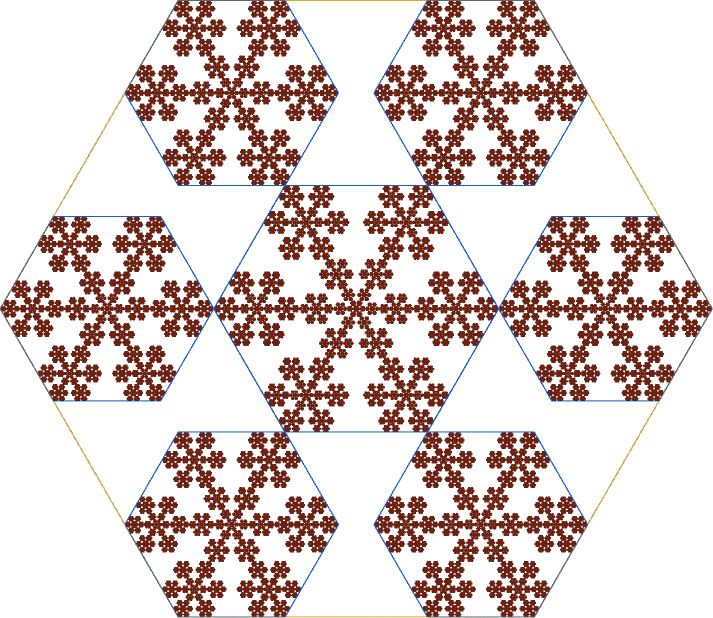
\includegraphics[width=1\linewidth]{14_6.png}
\caption{многоугольник -- шестиугольник} % подпись к рисунку
\label{ris146} % метка рисунка для ссылки на него  \ref{ris146}
\end{minipage}
\hfill
\begin{minipage}[h]{0.4\linewidth}
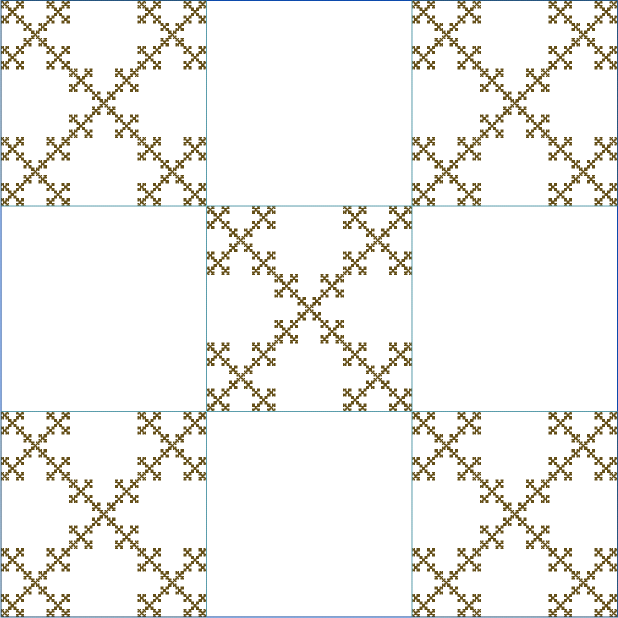
\includegraphics[width=1\linewidth]{14_7.png}
\caption{многоугольник -- квадрат}% подпись к рисунку
\label{ris147}% метка рисунка для ссылки на него  \ref{ris147}
\end{minipage}
\end{center}
\end{figure}

Этот метод позволяет построить лишь  простейшие примеры $G$-симмет\-рич\-ных $P$-полигональных систем. На самом же деле подобий исходного полиэдра, не касающихся своими вершинами вершин исходного многоугольника, может быть и более одного, требуется лишь выполнение условий {\bf (D1)-(D5)}. Более того, в множестве вершин  $\bigcup\limits_{i\in I}S_i(V_P)/V_P=\bigcup\limits_{i\in I}V_{P_i} / V_P$ могут попадаться вершины, общие сразу для трех и более копий многоугольников (в простом случае общей вершина бывает только для двух подобий полиэдров). Пример такой симметричной полигональной системы и её аттрактор показан на рисунке  \ref{ris145}. % Сим ПС из треугольников из презентации Мари


\begin{figure}[h!]
\begin{center}
\begin{minipage}[h]{0.45\linewidth}
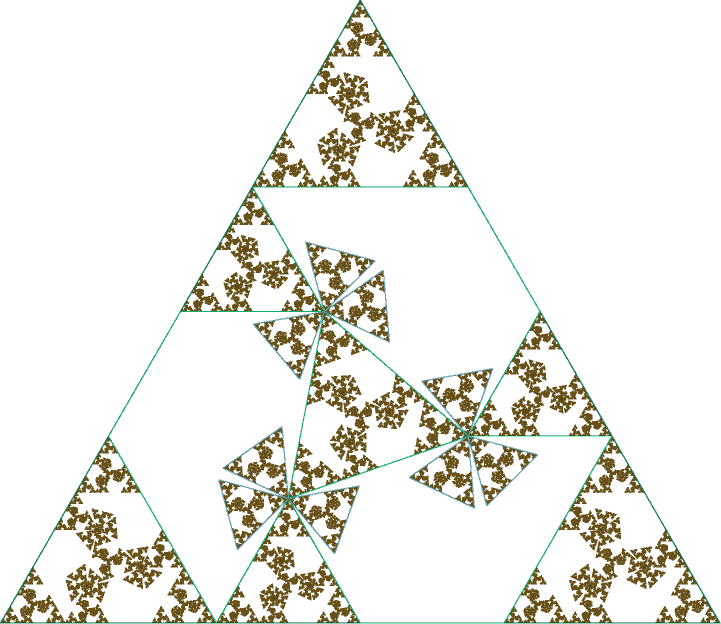
\includegraphics[width=1\linewidth]{14_5.png}
\caption{полигон -- треугольник}% подпись к рисунку
\label{ris145}% метка рисунка для ссылки на него  \ref{ris145}
\end{minipage}
\hfill
\begin{minipage}[h]{0.4\linewidth}
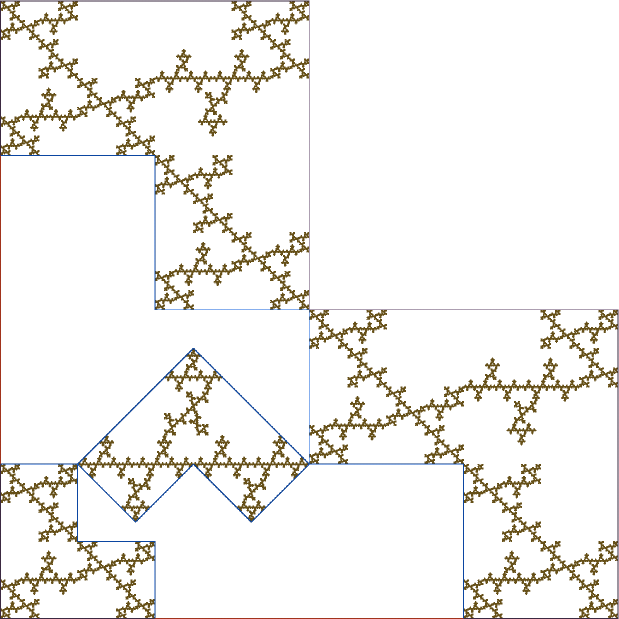
\includegraphics[width=1\linewidth]{14_3.png}
\caption{невыпуклый многоугольник} % подпись к рисунку
\label{ris143} % метка рисунка для ссылки на него  \ref{ris143}
\end{minipage}
\end{center}
\end{figure}

При построении стягиваемых $P$-полигональных систем (не симметричных) ограничений ещё меньше. Многоугольники в этом случае не обязаны быть правильными и выпуклыми (пример на рисунке \ref{ris143}). 

Теперь уже во всём множестве вершин $\bigcup\limits_{i\in I}V_{P_i}$ могут попадаться вершины, общие сразу для трех и более копий многоугольника  (примеры на рисунках \ref{ris148} и \ref{ris144}).

\begin{figure}[h]
\centering
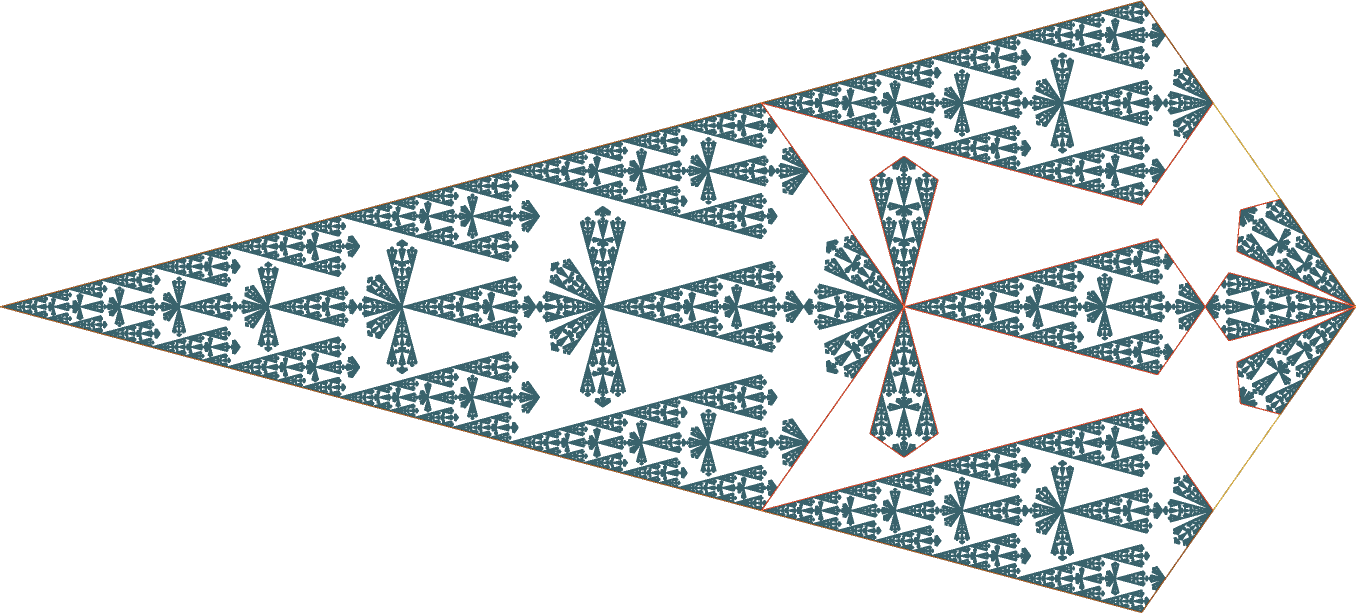
\includegraphics[width=0.95\textwidth]{14_8.png}
\caption{вершина многоугольника общая для трех подобий}% подпись к рисунку
\label{ris148}% метка рисунка для ссылки на него  \ref{ris148}
\end{figure}

\begin{figure}[h]
\centering
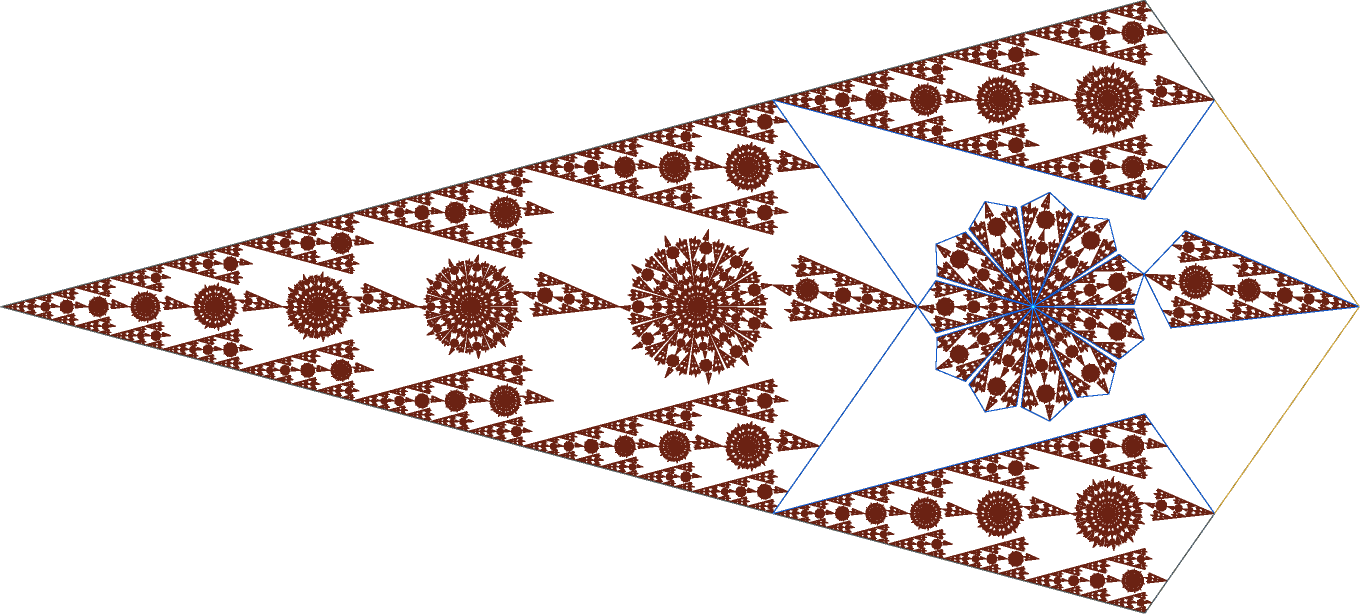
\includegraphics[width=1\textwidth]{14_4.png}
\caption{общая точка для 11 подобий}% подпись к рисунку
\label{ris144}% метка рисунка для ссылки на него  \ref{ris144}
\end{figure}

Подобие может содержать сразу несколько вершин исходного многоугольника, из-за чего может получиться полигональная система всего из двух подобий. Примеры полигональных систем из двух подобий и их аттракторы продемонстрированы на рисунках \ref{ris141} и \ref{ris142}, а на рисунке \ref{hata} продемонстрирован ещё один примечательный пример, называемый деревом Хаты, исходным многоугольником которого является семиугольник. Однако стоит отметить, что пример на рисунке \ref{ris141} тоже можно представить как симметричную полигональную систему, группа симметрий которого состоит всего из одного элемента, из отражения.

\begin{figure}[h!]
\begin{center}
\begin{minipage}[h]{0.5\linewidth}
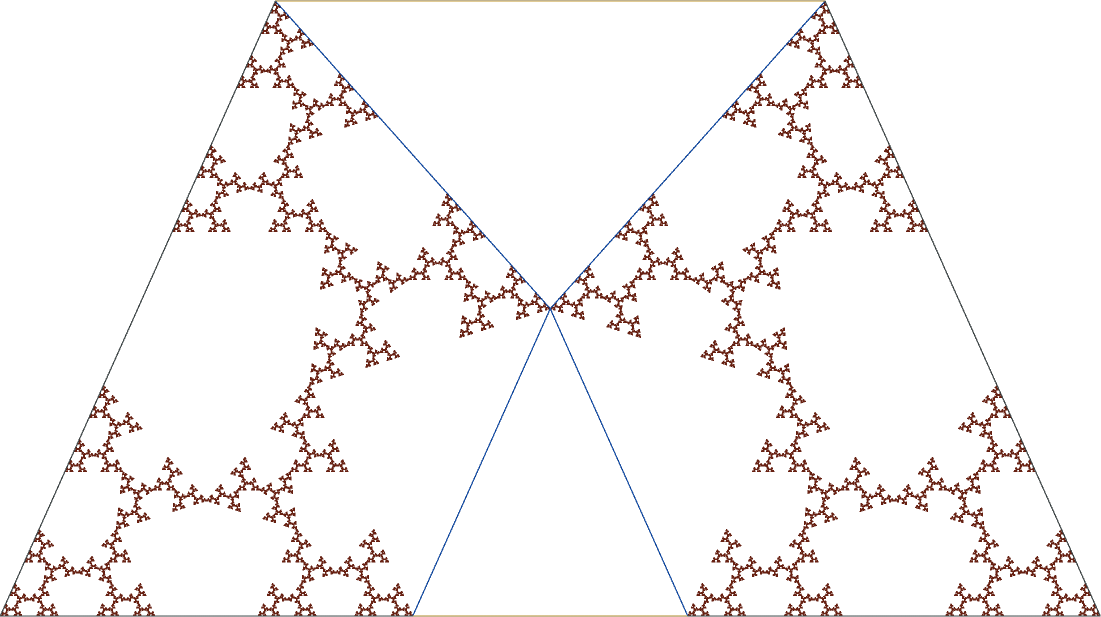
\includegraphics[width=1\linewidth]{14_1.png}
\caption{многоугольник -- равнобокая трапеция} % подпись к рисунку
\label{ris141} % метка рисунка для ссылки на него  \ref{ris141}
\end{minipage}
\hfill
\begin{minipage}[h]{0.4\linewidth}
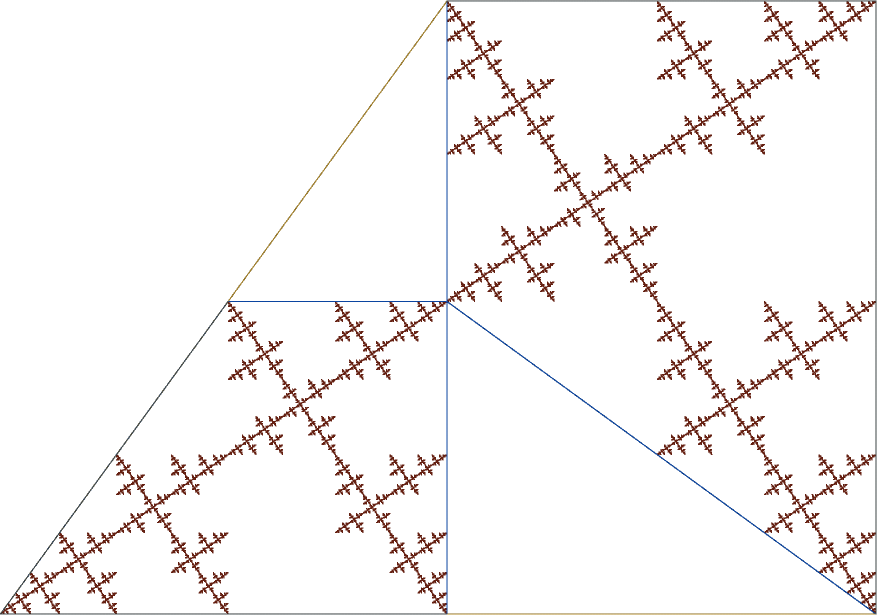
\includegraphics[width=1\linewidth]{14_2.png}
\caption{многоугольник -- трапеция}% подпись к рисунку
\label{ris142}% метка рисунка для ссылки на него  \ref{ris142}
\end{minipage}
\end{center}
\end{figure}

\begin{figure}[h]
\centering
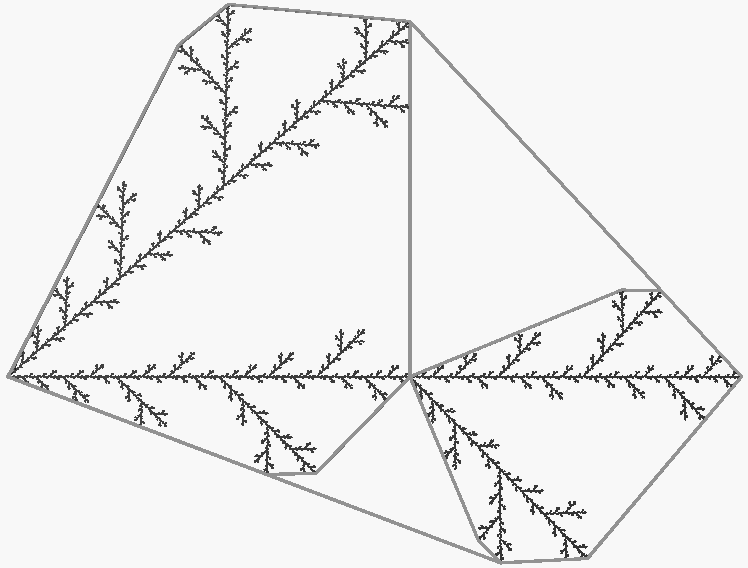
\includegraphics[width=0.8\textwidth]{hata3.png}
\caption{дерево Хаты}% подпись к рисунку
\label{hata}% метка рисунка для ссылки на него  \ref{hata}
\end{figure}

Если многоугольником является правильная фигура, то, используя повороты и отражения, подобие можно расположить на одной позиции сразу несколькими способами, тогда аттракторы полигональных систем при разных способах расположения и поворота подобий будут различаться (если это не симметричная полигональная система). На рисунках \ref{ris149} и \ref{ris1410} показаны примеры геометрически похожих полигональных систем, в которых по разному повернуто только самое маленькое подобие.

\begin{figure}[h!]
\begin{center}
\begin{minipage}[h]{0.48\linewidth}
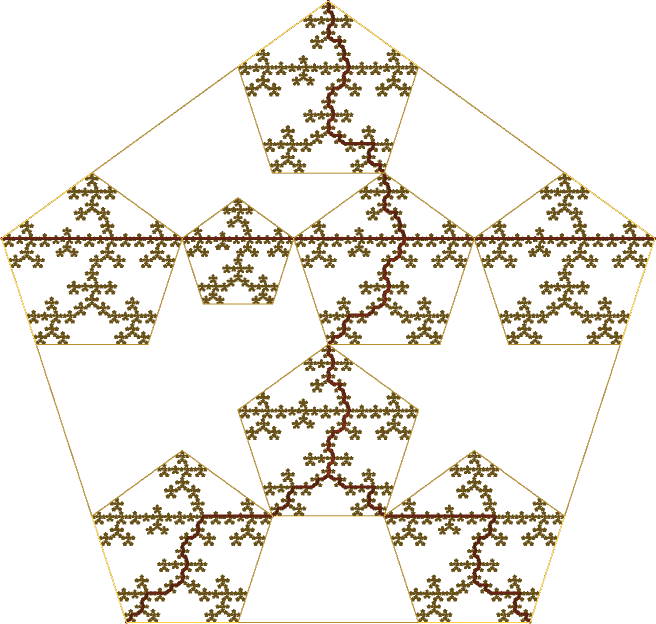
\includegraphics[width=1\linewidth]{14_9.png}
\caption{подобие в одном положении...} % подпись к рисунку
\label{ris149} % метка рисунка для ссылки на него  \ref{ris149}
\end{minipage}
\hfill
\begin{minipage}[h]{0.48\linewidth}
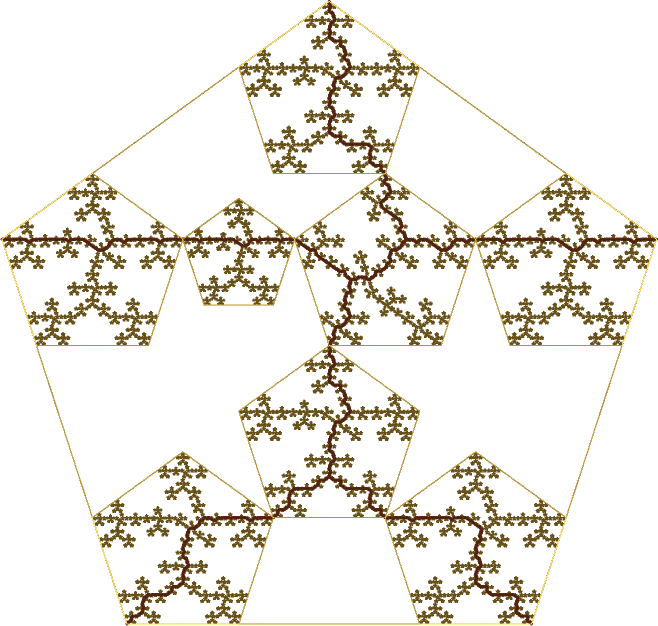
\includegraphics[width=1\linewidth]{14_10.png}
\caption{...а теперь в другом}% подпись к рисунку
\label{ris1410}% метка рисунка для ссылки на него  \ref{ris1410}
\end{minipage}
\end{center}
\end{figure}

При помощи стягиваемой полигональной $\eS$ системы мы можем построить циппер, удовлетворяющий условиям теоремы  \ref{zip1}. Для этого сперва выберем на исходном многоугольнике ребро $P'$, которое назовем основанием циппера. Далее, в маленьких многоугольниках выберем набор ребер, являющихся образами основания циппера. При этом отображения, переводящие основание циппера в выбранный набор ребер, должны представлять из себя композицию отображений из системы $\eS$ и поворотов из грцппы поворотов $G$ системы $\eS$ (только если $\eS$ -- симметричная). Сами же выбранные ребра должны образовывать ломаную, соединяющую начало и конец основания циппера. Получившаяся пара $(P',\eS')$ (где $\eS' = \{S_1',\ldots,S_m'\}$ -- это система отображений, перводящая основание циппера в вышеупомянутый набор ребер) и будет нужным нам циппером, аттрактор которого является дендритом и подконтинуумом аттрактора системы $\eS$. 

Ввиду введённых ограничений, наиболее удобно строить ципперы именно на симметричных полигональных системах, в которых используется правильный многоугольник и в группе поворотов которой достаточно поворотов и отражений. В противном же случае построить циппер возможно только тогда, когда геометрическая конфигурация стягиваемой полигональной системы позволяет перейти от одного маленького многоугольника к другому всего через одной ребро.

Используя на продемонстрированных на рисунке \ref{ris147} полигональной системе и аттракторе этот метод, мы можем построить следующий циппер и его аттрактор (который является дендритом и подконтинуумом дендрита на рисунке \ref{ris147}):

\begin{figure}[h!]
\begin{center}
\begin{minipage}[h]{0.48\linewidth}
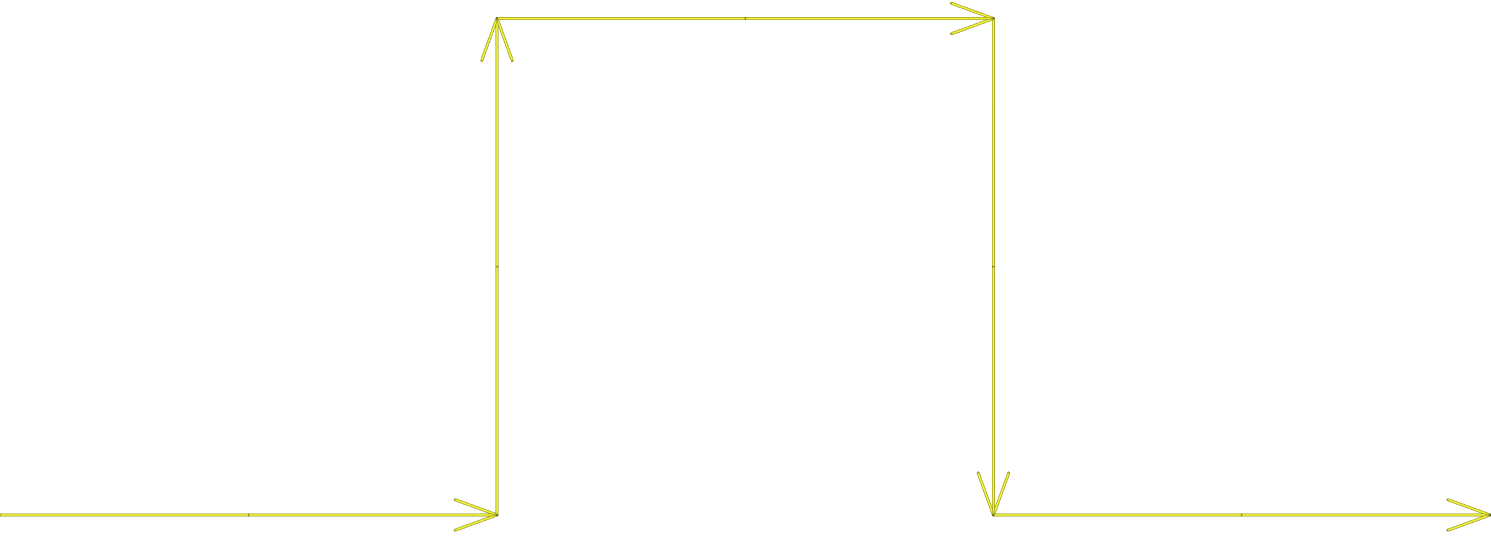
\includegraphics[width=1\linewidth]{zip1a.png}
\caption{Звенья циппера} % подпись к рисунку
\label{zip1a} % метка рисунка для ссылки на него  \ref{zip1a}
\end{minipage}
\hfill
\begin{minipage}[h]{0.48\linewidth}
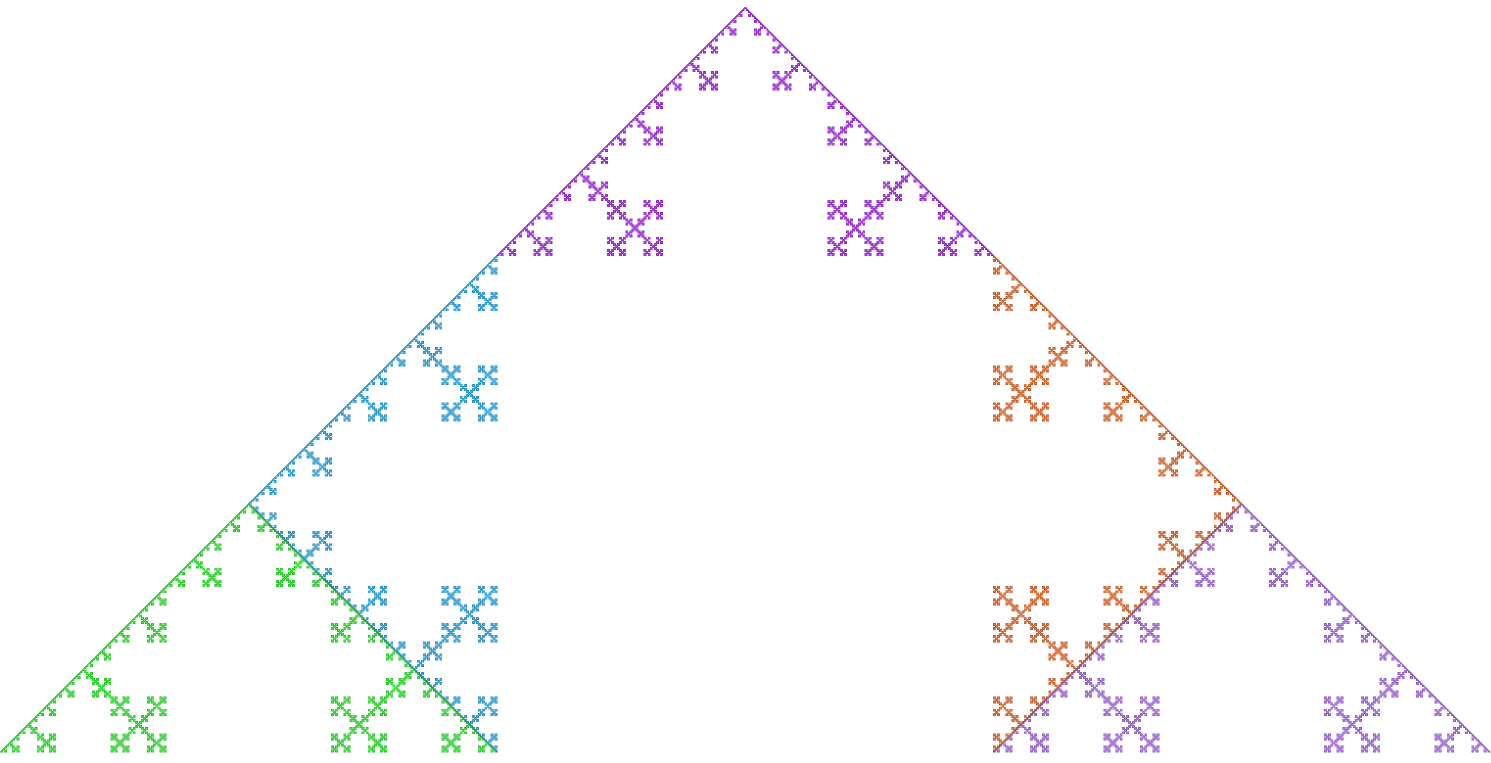
\includegraphics[width=1\linewidth]{zip1b.png}
\caption{Аттрактор циппера}% подпись к рисунку
\label{zip1b}% метка рисунка для ссылки на него  \ref{zip1b}
\end{minipage}
\end{center}
\end{figure}

Можно строить ципперы $\eS'$ полигональных систем $\eS$, аттракторы которых являются подконтинуумами аттракторов систем $\eS$, взяв вместо ребра многоугольника за основу циппера диагональ многоугольника. Все требования к ципперу и правила получения отображений остаются прежними, только теперь звеньями циппера должны быть такие же диагонали в выбранных подобиях, что и основание циппера, а цепочка звеньев циппера по-прежнему должна соединять начало и конец циппера. Пример такого циппера и его аттрактор приведен на рисунках \ref{ris1413}, \ref{ris1411} и \ref{ris1412}.

\begin{figure}[h]
\centering
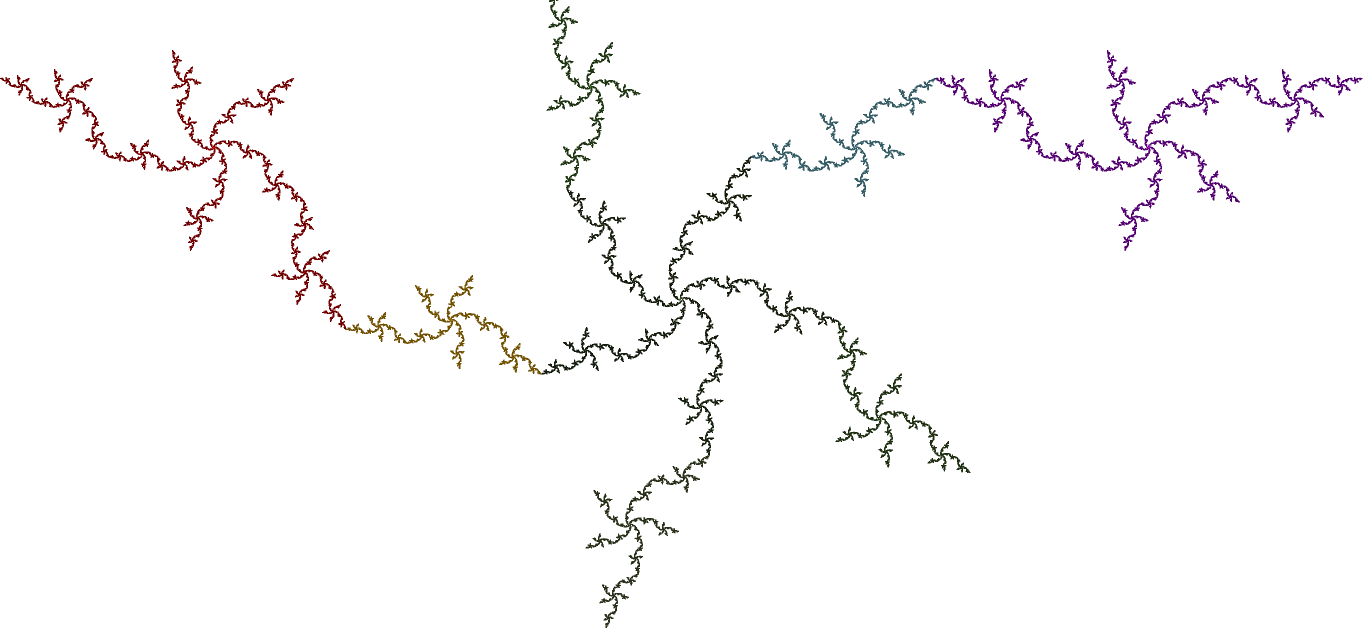
\includegraphics[width=0.85\linewidth]{14_13.png}
\caption{Аттрактор циппера}% подпись к рисунку
\label{ris1413}% метка рисунка для ссылки на него  \ref{ris1413}
\end{figure}

\begin{figure}[h!]
\begin{center}
\begin{minipage}[h]{0.49\linewidth}
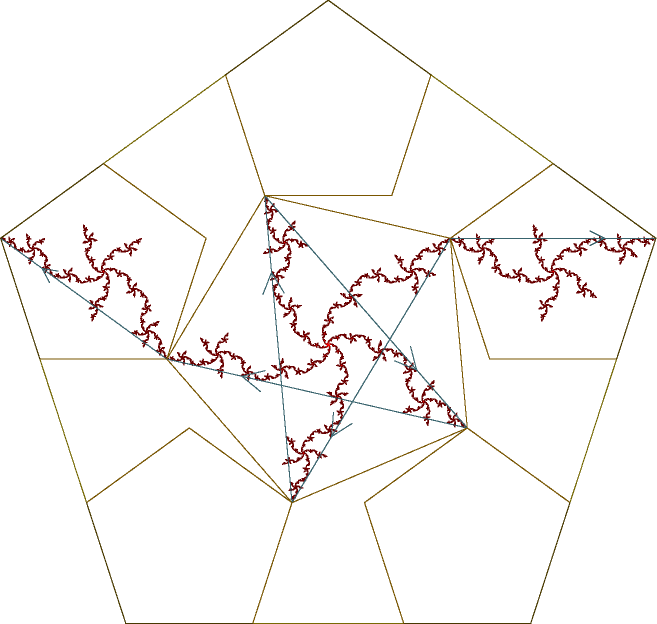
\includegraphics[width=1\linewidth]{14_11.png}
\caption{Звенья циппера и его аттрактор в полигональной системе} % подпись к рисунку
\label{ris1411} % метка рисунка для ссылки на него  \ref{ris1411}
\end{minipage}
\hfill
\begin{minipage}[h]{0.49\linewidth}
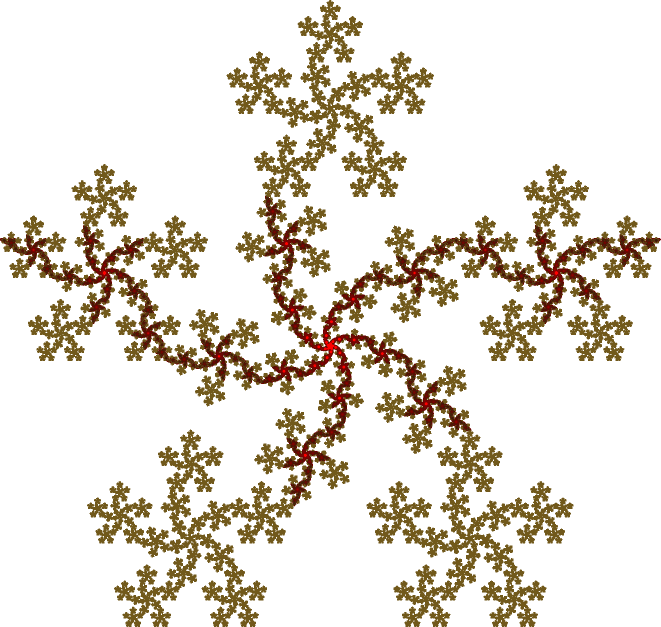
\includegraphics[width=1\linewidth]{14_12.png}
\caption{Аттрактор циппера является подконтинуумом аттрактора полигональной системы}% подпись к рисунку
\label{ris1412}% метка рисунка для ссылки на него  \ref{ris1412}
\end{minipage}
\end{center}
\end{figure}

\hspace{1cm}\\
\hspace{1cm}\\
\hspace{1cm}\\
\hspace{1cm}\\


%%%%%%%%%%%%%%%%%%%%%%%%%%%%%%%%%%%%%%%%%%%%%%%%%%%%%%%
%%%%%%%%%%%%%%%%%%%%%%%%%%%%%%%%%%%%%%%%%%%%%%%%%%%%%%%

\newpage
\section[Обобщенные полигональные системы]{ОБОБЩЕННЫЕ ПОЛИГОНАЛЬНЫЕ СИСТЕМЫ}

\subsection{Обобщенные полигональные системы}


Если мы опустим условие {\bf(D1)} в определении стягиваемой $P$-полигональной системы $\eS$, то получим определение {\em обобщенной $P$-полигональной системы}:
\begin{definition}\label{gps}
Система \ $\eS=\{S_1,...,S_m\} $, удовлетворяющая условиям {\bf D2-D4}, называется обобщенной $P$-полигональной системой подобий.
\end{definition}
\begin{figure}[h]
\centering
 \resizebox{0.9\textwidth}{!}{{\small\begin{tikzpicture}[line cap=round,line join=round,>=stealth ,x=10.0cm,y=10.0cm]
    \node  at (-.098,0.02) {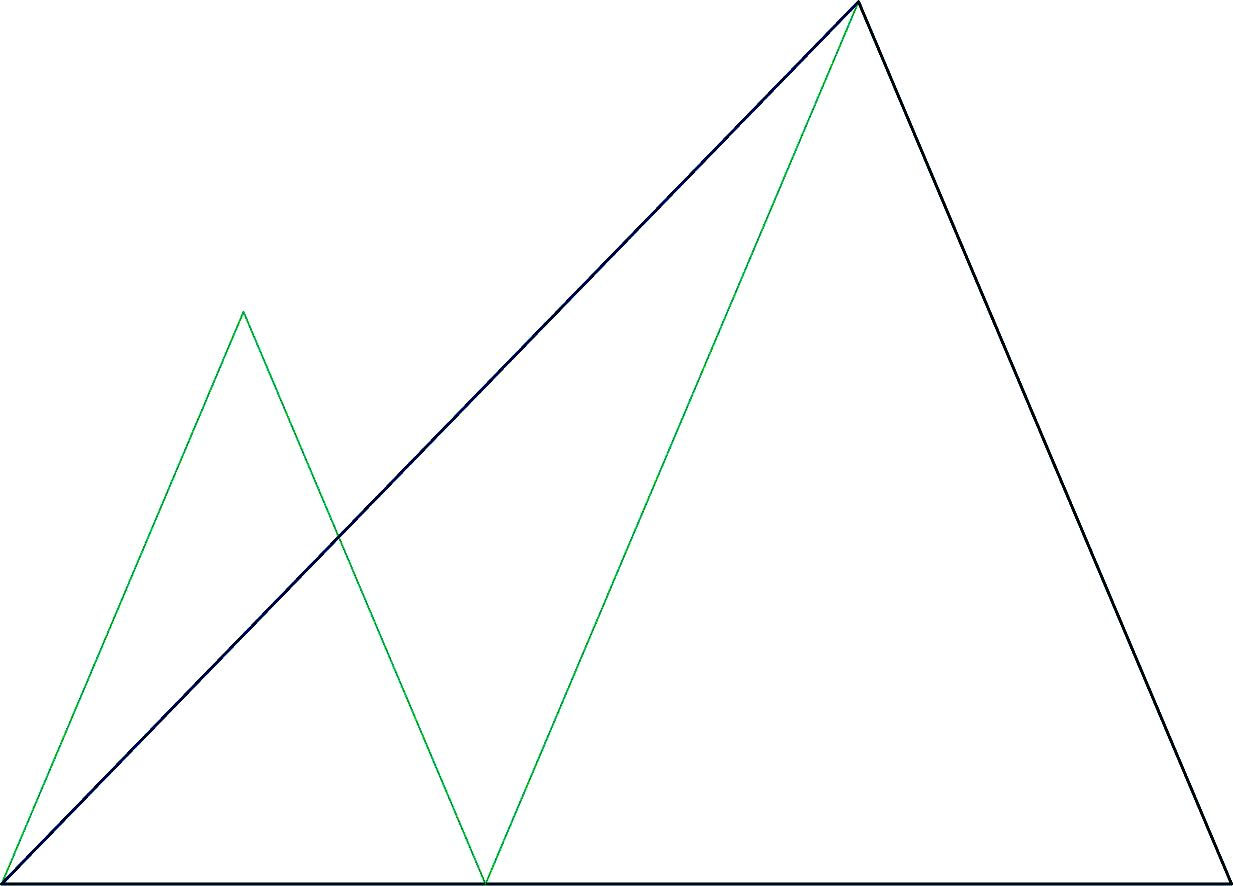
\includegraphics[width=.36\textwidth]{gps1.jpg} };
   \node  at (.65,-.01) {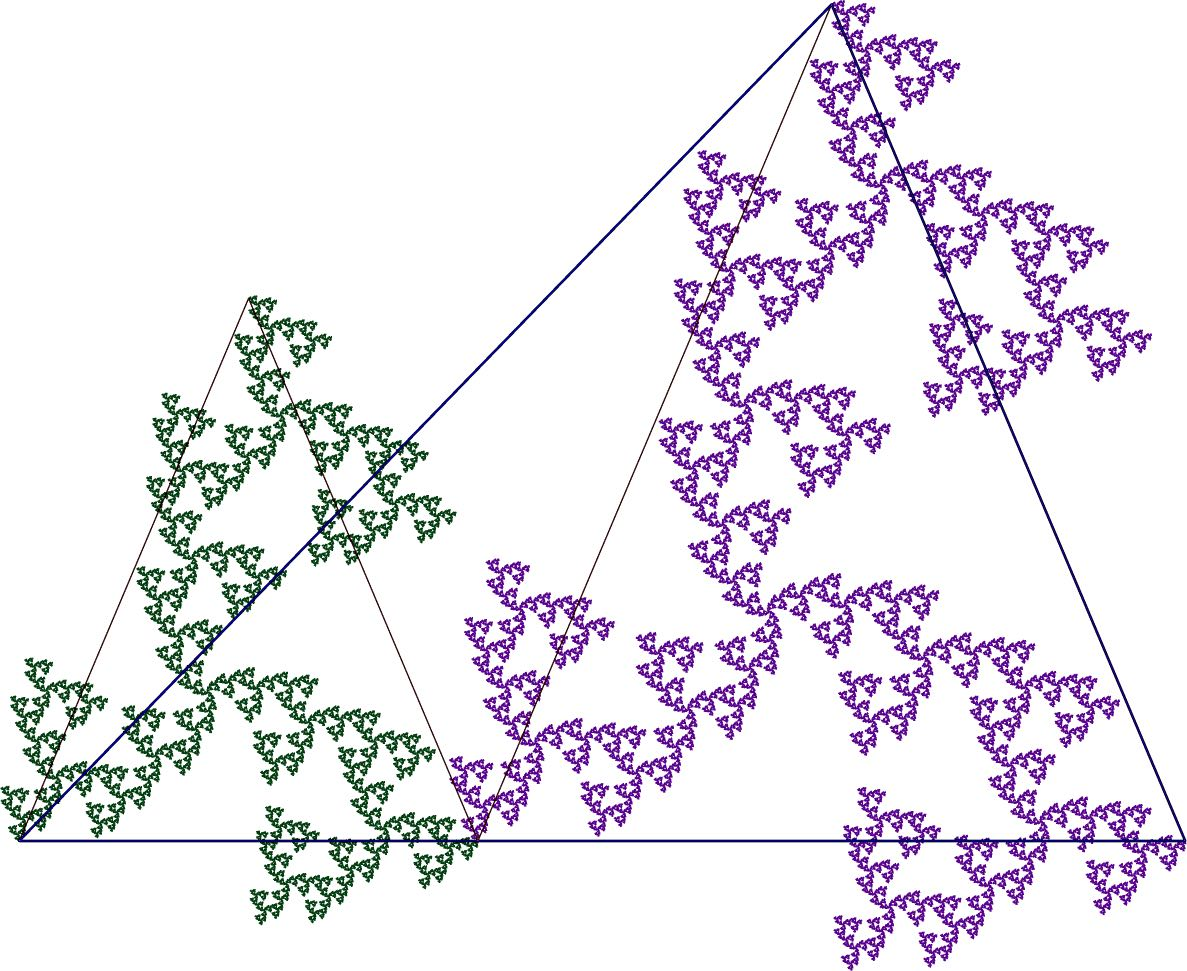
\includegraphics[width=.37\textwidth]{tyl.jpg}};
      \node at (0.02,0){$P_2$}; \node at (-0.14,-.02){$P$};\node at (-0.28,-0) {$P_1$};\node at (0.51,-.08) {$K_1$};\node at (.81,-.03){$K_2$};
\end{tikzpicture}}}
\caption{Обобщенная полигональная система и её аттрактор}% подпись к рисунку
\label{gps1}% метка рисунка для ссылки на него  \ref{gps1}
\end{figure}

Однако аттрактор такой обобщенной полигональной системы (ОПС) уже не обязательно будет дендритом. И может возникнуть справедливый вопрос: при каких же условиях аттрактор ОПС будет дендритом? И достаточное условие того, что аттрактор ОПС будет дендритом, всё же было найдено.

\begin{theorem}\label{pcint}
Пусть $\eS$ --- это обобщенная $P$-полигональная система.  Если для любых $i, j \in I$ \begin{equation}\label{icnd}S_i(K)\cap S_j(K)=P_i\cap P_j,\end{equation} то аттрактор $K$ системы $\eS$ является дендритом.
\end{theorem}
 
Для доказательства этой теоремы есть несколько подходов. В статье А.В.~Тетенова \cite{FPS}, например, представлен обобщенный аналог этой теоремы, который мы далее и рассмотрим. Но сперва введем некоторые определения.

Мы начнем с определения систем множеств с FIP.
\begin{definition}\label{fipss}
Будем говорить, что система компактных множеств  $\eA=\{A_i,i\in I\}$ в топологическом пространстве $X$ является системой с конечным  (соотв. одноточесным) пересечением, если для любых  $i\neq j\in I $ пересечение $P_{ij}=A_i\cap A_j$ is конечно (соотв. не более чем одноточечно).\\
\end{definition}

Тогда мы говорим, что $\eA$ -- это {\em система множеств с  FIP (соотв. FIP1)}.\\ 
 
Пусть $A=\bigcup\limits_{A_i\in I}A_i$ и  $P=\bigcup\limits_{i\neq j}P_{ij} $. Мы также обозначим $P_i=\bigcup\limits_{j\neq i}P_{ij}$. 

Для каждой системы множеств с FIP мы определяем ее граф пересечения:
\begin{definition}\label{igraph}
Граф пересечений  $\Ga(\eA)$ системы множеств с FIP $\eA$ --- это двудольный граф  $(P,\eA; E)$, для которого  $\{A_i,p\}\in E$ тогда и только тогда, когда $p\in A_i$. 
\end{definition}

Мы называем $A_i\in \eA$ {\em белыми вершинами} , а $p\in P$ -- {\em черными вершинами}.  Множество $N(A_i)$ черных вершин, смежных к белой вершине $A_i$ совпадает с   $P_i$, тогда как для черной вершины $p$,  $N(p)=\{A_i:p\in A_i\}$. Поскольку $p$ является точкой пересечения по крайней мере двух множеств $A_i$, \quad $ \mathrm{deg}(p)\ge 2$.\\
 
Основное применение этих определений относится системам сжимающих отображений и их аттракторам.
Пусть $\eS=\{S_1,...,S_m\}$ -- система сжимающих отображений в полном метрическом пространстве $X$, а $K$ --- её аттрактор. Пусть $\eA(\eS)=\{K_1,..., K_m\}$ и $\eA_n(\eS)=\{K_\bi:\bi\in I^n\}$.
 
\begin{definition}\label{fipcs}
 $\eS$ называется FIP-системой сжатий  (соотв. FIP1-системой сжатий), если система $\eA(\eS)$ является FIP-системой множеств (соотв. FIP1-системой множеств).
\end{definition}

Если граф пересечений $\Ga(\eA)$  FIP-системы множеств с является деревом, то $\eA$ -- это FIP1-система (или система множеств с одноточечным пересечением).

Если граф пересечения FIP1-системы множеств  $\eA$ является деревом, то простая петля в $A$ не может пересечь ни одной из границ между множествами $A_i$:

\begin{prop} 
Пусть $\eA$ --- это FIP1-система множеств и $\Ga(\eA)$ является деревом. Пусть $\ga$ --- простая замкнутая кривая в $A$. Тогда существует единственное множество $A_k\in\eA$ такое, что $\ga\IN A_k$.
\end{prop}

\dok Не ограничивая общности, мы можем предполагать, что все множества  $A_i$ связны. Пусть $p$ -- некоторая точка в $P$ и пусть $Q_i,Q_j$ -- это компоненты $A\mmm\{p\}$. Предположим, что $\ga$ -- это замкнутая кривая, содержащая некоторые $a\in Q_i$ и $b\in Q_j$. Поскольку каждый путь, соединяющий $a$ и $b$, проходит через $p$, точка $p$ является кратной точкой $\ga$. следовательно если $\ga\cap  \dot A_i$, то $\ga\in A_i$.\vse

\begin{theorem}
Пусть $\eS$ -- такая система иньективных сжимающих отображений в полном метрическом пространстве $X$ , что её граф пересечений $\Ga_1(\eS)$ является деревом. Тогда аттрактор $K$ системы $\eS$ будет дендритом.
\end{theorem}

\dok Пусть $\ga\in K$ -- простая замкнутая кривая. Поскольку для любого $n\in \nn$ граф $\Ga_n$ является деревом, то существует единственный $\bj\in I^n$ такой, что $\ga\in K_\bj$. Следовательно $|\ga|=0$. \vse\\

Используя эту теорему, доказательство Теоремы \ref{pcint} будет очевидным. Действительно, из формулы (\ref{icnd}) становится понятно, что графы пересечений $\Ga(\{K_i\})$ и $\Ga(\{P_i\})$ совпадают. А благодаря свойствам {\bf (D2)-(D4)} обобщенной полигональной системы граф пересечений $\Ga(\{P_i\})$ --- дерево. А значит  Теорема \ref{pcint} справедлива.

\begin{corollary}
Пусть $\eS$ -- обобщенная $P$-полигональная система, удовлетворяющая условию (\ref{icnd}). Для любой поддуги $\ga_{xy}\IN K$ и для любого $n$ существует единственная цепочка попарно различных мультииндексов $\bi_1,\bi_2,...,\bi_l\in I^n$, которая разбивает $\ga_{xy}$ на последовательные поддуги \\ $\ga_{xx_1}\IN K_{i_1},\ldots,\ \ga_{x_{k-1}x_k}\IN K_{i_k},\ldots,\ \ga_{x_{l-1}y}\IN K_{i_l}$.\vse
\end{corollary}

\begin{rmk} 
Обобщенная $P$-полигональная система $\eS$ может не удовлетворять условию (\ref{icnd}) и иметь аттрактор $K$, являющийся дендритом. Аттрактор $K$ обобщенной полигональной системы $\eS$ на рисунке ниже является дендритом, но  $P_7\cap P_9=\0$,тогда как $K_7\cap K_9$ -- это отрезком прямой.
\end{rmk}

\begin{figure}[h!]
\centering
\resizebox{1\textwidth}{!}{{\begin{tikzpicture}[line cap=round,line join=round,>=stealth ,x=10.0cm,y=10.0cm]
\node[anchor=south west,inner sep=0] at (0,-.227) {
   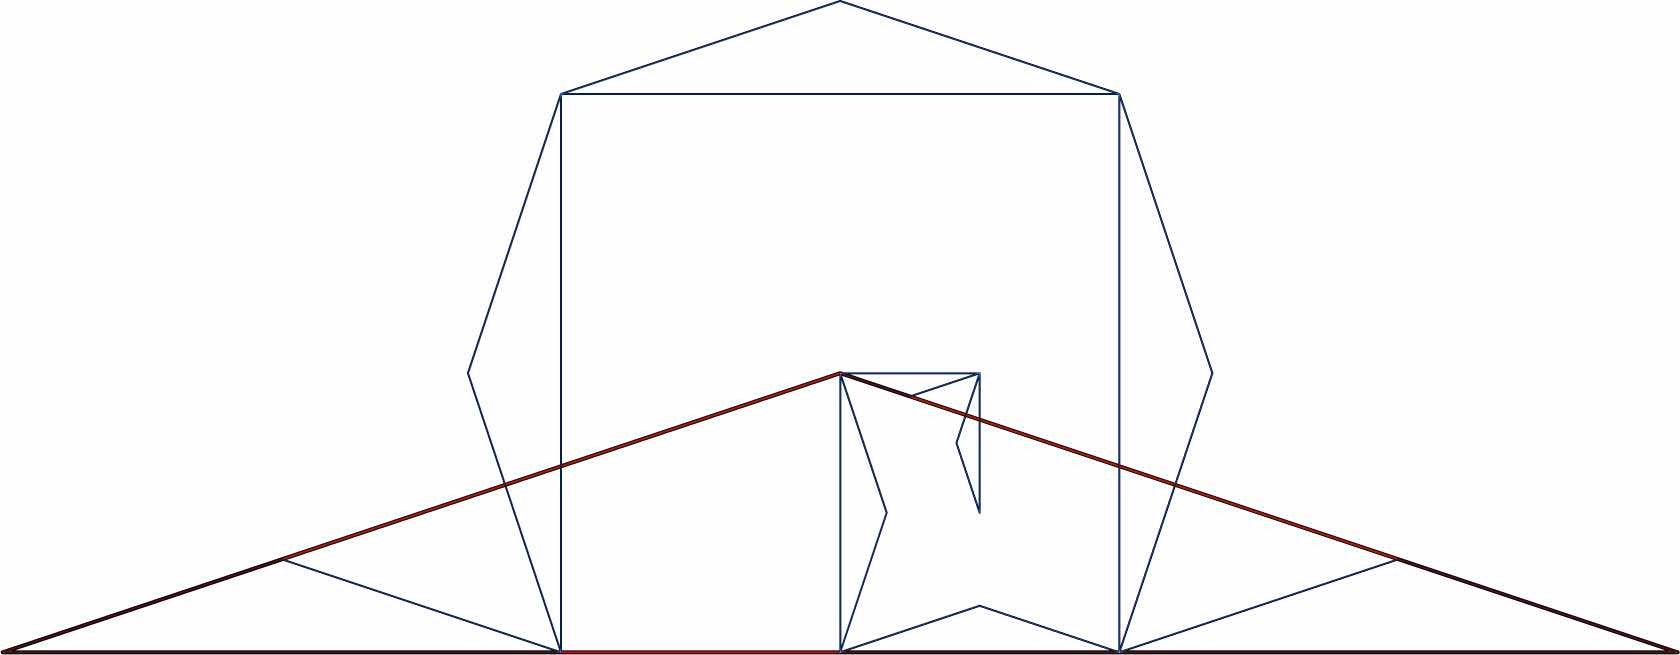
\includegraphics[width=.45\textwidth]{cntrex0.jpg}\quad  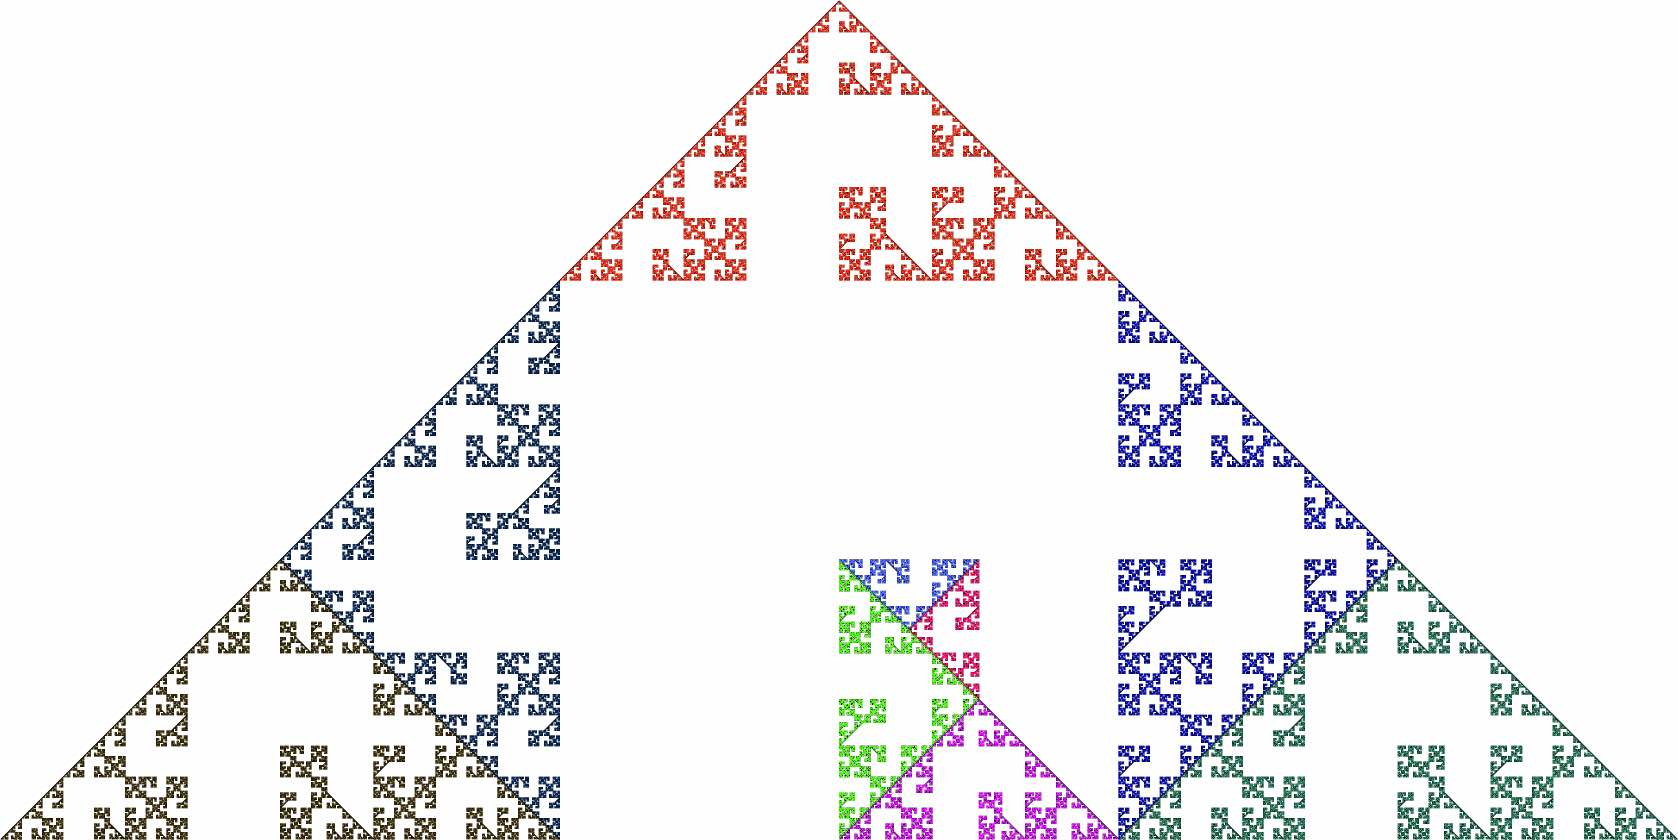
\includegraphics[width=.45\textwidth]{cntrex.jpg}}; 
\draw (0.13,-0.25) node {$P_1 $} (0.18,-0.1) node  {$P_2 $} 
(0.37,0) node {$P_3 $}(0.58,-0.1) node  {$P_4 $} (0.64,-0.25) node {$P_5 $} (0.44,-0.25) node {$P_6 $} (0.35,-0.17) node {$P_7 $} (0.41,-0.07) node {$P_8 $} (0.47,-0.16) node {$P_9 $};
\draw (.94,-0.25) node {$K_1 $} (0.98,0) node  {$K_2 $} 
(1.18,0) node {$K_3 $}(1.39,0) node  {$K_4 $} (1.45,-.25) 
node {$K_5 $} (1.26,-0.25) node {$K_6 $} (1.155,-0.17) node {$K_7 $} (1.22,-0.07) node {$K_8 $} (1.275,-0.14) node {$K_9 $};
\end{tikzpicture}}}
 \caption{}% подпись к рисунку
\label{cntrex}% метка рисунка для ссылки на него  \ref{cntrex}
\end{figure}

Так или иначе, чтобы воспользоваться на практике Теоремой \ref{pcint} и формулой (\ref{icnd}), необходимо построить аттрактор, что будет не совсем корректно с точки зрения постановки задачи. Нам нужно проверить дендритность атррактора, имея на руках только систему сжимающих отображений. С учетом того, что нас интересует проверка дендритности не всех обобщенных полигональных систем, а их конкретного подкласса (т.е. $\da$-деформаций стягиваемых полигональных систем, о которых в следующем пунке), то Теорема \ref{pcint} и формула (\ref{icnd}) нам еще пригодятся.%Зачем я написал этот абзац? Может убрать?


\subsection{ $\da$-деформации стягиваемых полигональных систем.}

\begin{definition}\label{deform} 
Пусть $\da>0$. Обобщенная $P'$-полигональная система $\eS'=\{S'_1,...,S'_m\}$ называется $\da$-деформацией $P$-полигональной системы $\eS=\{S_1,...,S_m\}$, если существует биекция $f:\bigcup\limits_{k=1}^m \eV_{P_k}\to \bigcup\limits_{k=1}^m \eV_{P'_k}$ такая, что\\
a) $f|_{\eV_P}$ продолжается до гомеоморфизма $\tilde f: P\to  P'$; \\ b) $|f(x)-x|<\delta$  для любого $x\in \bigcup\limits_{k=1}^m \eV_{P_k}$\\  c) $f(S_k(x))=S'_k(f(x))$ для любого $k\in I$ и $x\in \eV_P$.\bigskip
\end{definition}

\begin{figure}[h!]
\centering
\resizebox{1\textwidth}{!}{{
\begin{tikzpicture}[x=10.0cm,y=10.0cm]
\node[anchor=south west,inner sep=0] at (0,0) {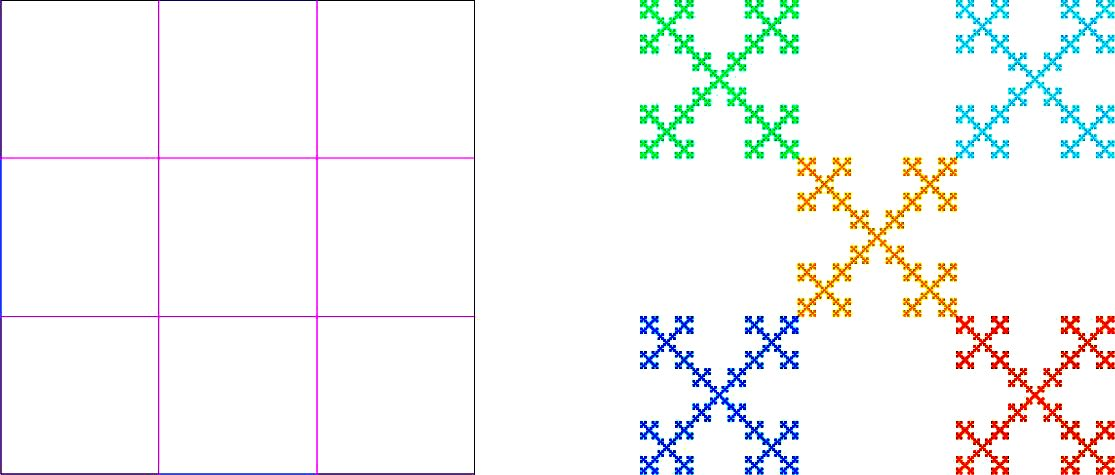
\includegraphics[width=.43\textwidth]{def0.jpg}};
 \node[anchor=south west,inner sep=0] at (0.85,-.03){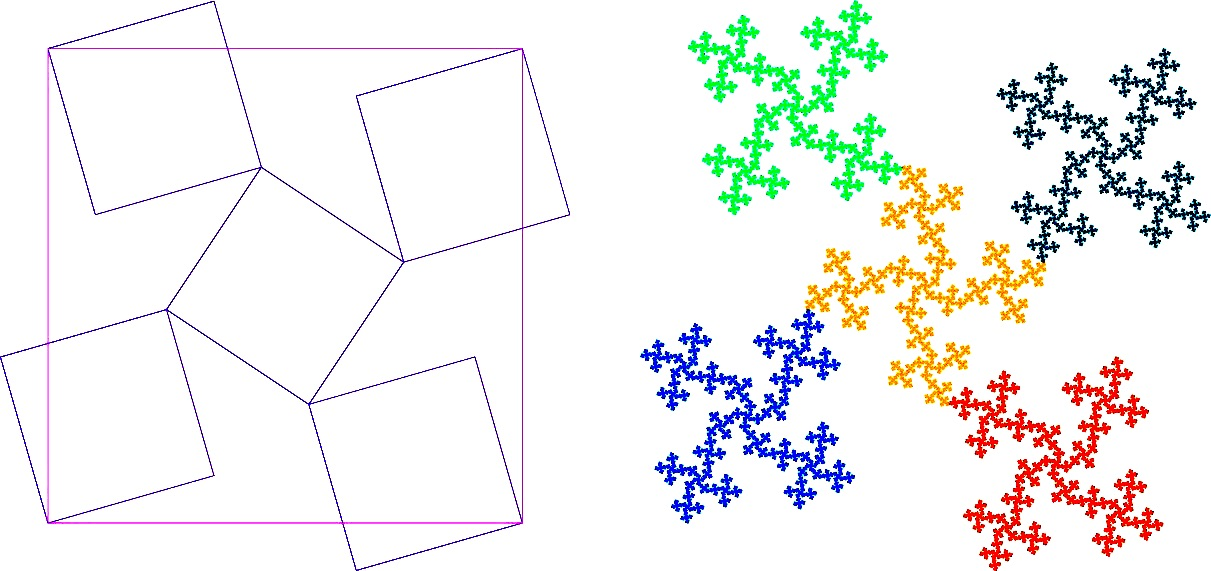
\includegraphics[width=.47\textwidth]{def2.jpg}};
    %\draw[step=.01,yellow,very thin] (0,-.1) grid (1.7,.35);
  % \draw[step=.1,green,very thin] (0,-.1) grid (1.7,.35);
    \node at(0.27,.25){$P_3$}; \node at (.15,.15) {$P_5$};\node at (.27,.05) {$P_2$};\node at (.05,.25) {$P_4$};\node at (0.05,.05) {$P_1$};
\node at (1.15,.24){$P'_3$}; \node at (1.05,.15) {$P'_5$};\node at (1.12,0.03) {$P'_2$};\node at (0.94,.27) {$P'_4$};\node at (.93,.06){$P'_1$};

\end{tikzpicture}}}
\caption{Полигональная система $\eS$ и её $\da$-деформация $\eS'$}% подпись к рисунку
\label{cntrex}% метка рисунка для ссылки на него  \ref{cntrex}
\end{figure}

Обратите внимание, что по Определению \ref{deform} если $z_1,z_2\in \eV_P$, $i,j\in I$  и $S_i(z_1)=S_j(z_2)$, то $S'_i( f(z_1))=S'_j(f(z_2))$.  Кроме того, мы имеем следующее
\begin{lemma}\label{bibj}
%If $A_1,A_2\in \eV_P$, $\bi,\bj\in\ia$ and $S_\bi(A_1)=S_\bj(A_2)$, then $S'_\bi( f(A_1))=S'_\bj( f(A_2))$.
Если $A_1,A_2\in \eV_P$, $\bi,\bj\in\ia$ и $S_\bi(A_1)=S_\bj(A_2)$, то $S'_\bi( f(A_1))=S'_\bj( f(A_2))$.
\end{lemma}
 
\dok
Предположим, что $S_\bi(A)=B\in \eV_\wP$ для некоторого $A\in \eV_P$, и пусть $\bi=i_1i_2...i_n$. Обозначим $S_{i_{k+1}...i_n}(A)$ как $A_k$.

Тогда мы имеем конечную последовательность соотношений между $B\in \eV_\wP$ и вершинами $A_k\in\eV_P$:\\
\beq\label{chn1} B=S_{i_1}(A_1); \quad A_1=S_{i_2}(A_2); \quad \ldots A_{n-1}=S_{i_n}(A)\eeq
Поскольку, по c), $f(S_k(A_k))= S'_k(A'_k)$, \qquad $A'_{k-1}=f(A_{k-1})=f(S_k(A_k))=S'_k(A'_k)$, то отображение $f$ преобразует соотношения \ref{chn1} в  
\beq\label{chn2} B'=S'_{i_1}(A'_1); \quad A'_1=S'_{i_2}(A'_2); \quad \ldots  A'_{n-1}=S'_{i_n}(A'),\eeq
поэтому $S'_\bi(A')=B'$\\
Поэтому если $S_\bi(A_1)=S_\bj(A_2)\in \eV_{\wP}$, то $S'_\bi(f(A_1))=S'_\bj(f(A_2))$. \\

 
Теперь предположим, что $S_\bi(A_1)=S_\bj(A_2)$ и $\bi=\bl\bi'$, $\bj=\bl\bj'$ и $S_\bi(A_1)=S_\bj(A_2)=S_\bl(B)$ для некоторого $B\in \eV_\wP$. Тогда  $S_{\bi'}(A_1)=S_{\bj'}(A_2)=B$, следовательно $S'_{\bi'}(f(A_1))=S'_{\bj'}(f(A_2))=f(B)$ и
$S'_{\bi}(f(A_1))=S'_{\bj}(f(A_2))=S'_\bl(f(B))$. \vse\\

\begin{theorem}\label{attrmap}
Пусть $K$ и $K'$ -- аттракторы стягиваемой $P$-полигональной системы $\eS$ и её $\da$-деформации $\eS'$ соответственно, а $\pi:I^\8\to K,\pi':I^\8\to K'$ -- соответствующие индексные отображения.\\ (i)  Существует единственное непрерывное отображение $\hat f:K\to K'$ такое, что $\hat f\circ\pi=\pi'$.\\ (ii) Если $\eS'$ удовлетворяет условию \ref{icnd}, то $\hat f$ является гомеоморфизмом.
\end{theorem}

\begin{rmk}
Эквивалентная формулировка утверждения (i) Теоремы такова:\\{\em Существует единственное непрерывное отображение $\hat f:K\to K'$ такое, что для любого $z\in K$ и $\bi\in\ia$,}
\beq\label{compat}\hat f(S_\bi(z))=S'_\bi(\hat f(z)).\eeq
\end{rmk}

\dok
Доказательство анологично (см.\cite[Lemma 1.]{ATK}). Во-первых, мы определим функцию $\hat f$, которая является сюрьекцией плотного подмножества $G_\eS(\eV_P)\IN K$ в плотное подмножество $G_{\eS'}(\eV_{P'})\IN K'$. Во-вторых, мы покажем, что она непрерывна по Гёльдеру на $G_\eS(\eV_P)$, и, следовательно, имеет единственное непрерывное продолжение до сюрьекции из $K$ в $K'$, которое мы обозначим для прежднего символа как $\hat f$. В-третьих, мы покажем, что условие \ref{icnd} подразумевает, что $\hat f$ является инъективным и поэтому является гомеоморфизмом..\\

%1. Define a map $\hat f(z):G_\eS(\eV_P)\to G_{\eS'}(\eV_{P'})$ by:
1. Определим отображение $\hat f(z):G_\eS(\eV_P)\to G_{\eS'}(\eV_{P'})$ как
\beq\label{hatf}\hat f(z)=S'_\bi(f(S_\bi^{-1}(z))\mbox{,  где   }z\in S_\bi(\eV_P)\eeq
Как следует из Леммы \ref{bibj}, если $S_\bi(A_1)=S_\bj(A_2)=z$, то $S'_\bi(f(S_\bi^{-1}(z)))=S'_\bj(f(S_\bj^{-1}(z)))$, поэтому отображение $\hat f$ корректно определено.

Очевидно, что $\hat f(G_\eS(\eV_P))= G_{\eS'}(\eV_{P'})$, потому что если $A'\in \eV_{P'}$ и $z'=S'_\bi(A')$, то существует вершина $A=f^{-1}(A')\in \eV_P$, вследствие этого $z'=\hat f(S_\bi(A))$.

Кроме того, для любого  $z\in G_\eS(\eV_P)$ и $\bi\in\ia$, $\hat f(S_\bi(z))=S'_\bi(\hat f(z))$ и\\ если $z_1,z_2\in G_\eS(\eV_P)$, $\bi,\bj\in\ia$ и $S_\bi(z_1)=S_\bj(z_2)$, то $S'_\bi(\hat f(z_1))=S'_\bj(\hat f(z_2))$.\\

2. Пусть $q_k = \Lip S_k$, $q_k' = \Lip S_k'$,  $\beta = \min \limits _{k\in I } {\dfrac {\log {q'_k}} {\log {q_k}}}$.\\

Затем, следуя доказательству \cite[Теорема 27, step 4.]{TSV0}, в котором для наших оценок мы используем $K'$ вместо $P'$, мы видим, что для любых $z_1,z_2\in G_\eS(\eV_P)$,
$$|z_1'-z_2'| \le\dfrac {2|K'|} {(\rho_0\cdot\sin {(\al_0/2)})^{\beta}}|z_1-z_2|^{\beta}.$$
   
Поэтому отображение $\hat f$ может быть расширено до непрерывного по Гёльдеру сюрьективного отображения множества $K$ в $K'$. Поскольку для любого $z\in K$ и любого $k\in I$ справедливо $\hat f(S_k(z))=S'_k(f(z))$, то $\hat f\circ\pi=\pi'$.\\
 
3. Теперь предположим, что система $\eS'$ удовлетворяет условию (\ref{icnd}). Предположим, что для некоторых $\bm\sa=i_1i_2...\in I^\8$ и $\bm\tau=j_1j_2...\in I^\8$ справедливо $\hat f\circ\pi(\bm\sa)=\hat f\circ\pi(\bm\tau)$. Тогда, если $i_1\neq j_1$, то, по условию \ref{icnd}, $P'_{i_1}\cap P'_{j_1}\neq\0$, в результате чего   $P_{i_1}\cap P_{j_1}=\{B\}$ для некоторого $B\in \eV_\wP$ и $\pi(\bm\sa)=\pi(\bm\tau)=B$.
 
Пусть теперь  $\bm\sa=\bl\bm\sa'$ и $\bm\tau=\bl\bm\tau'$, а $\hat f\circ\pi(\bm\sa)=\hat f\circ\pi(\bm\tau)$. Тогда, по формуле \ref{compat}, $\hat f\circ\pi(\bm\sa')=\hat f\circ\pi(\bm\tau')$, так что если первые индексы в $\bm\sa'$ и  $\bm\tau'$ различны, то $\pi(\bm\sa)=\pi(\bm\tau)=S_\bl(B)$ для некоторого $B\in \eV_\wP$. 
 
Это подразумевает иньективность отображения $\hat f$. Таким образом $\hat f$ -- гомеоморфизм компактных множеств $K$ и $K'$. \vse\\

\subsection{Циклические вершины и теорема о совпадении параметров}

\begin{definition}\label{cyclic}
Пусть $\eS$ является стягиваемой $P$-полигональной системой подобий.
Вершина $A \subset \eV_P$ называется циклической вершиной, если существует такой мультииндекс  $\bi=i_1 i_2 \ldots i_k$, что $S_\bi(A)=A$. 
Наименьшее число $k=|\bi|$ среди всех $\bi$, для которых $S_\bi(A)=A$, называется {\em порядком} циклической вершины $A$.
\end{definition}

\begin{definition}
Точка $B \in\cup_{i=1}^m  \eV_{P_i}$ подчинена циклической вершине  $A$, если для некоторого мультииндекса $\bi, S_{\bi}(A)=B$.
\end{definition}

\begin{prop}\label{1ordcyc}
Пусть $\eS$ --- стягиваемая $P$-полигональная система подобий. тогда:\\
(1) Всякая вершина $B\in \eV_P$ подчинена некоторой циклической вершине.\\
(2) Существует такой $n$, что в системе $\eS^{(n)}=\{S_\bi, \bi\in I^n\}$ все циклические вершины имеют порядок 1.
\end{prop}

{\bf Доказательство.} 
Обратим внимание, что если $A\in \eV_P$ --- циклическая вершина, то существует такой мультииндекс $\bj\in\ia$, что $S_\bj(A)=A$. 
Следовательно, если для некоторых $\bj\in\ia$, $ A\in P_\bj$, то для некоторого $n$, $S_\bj^n(P)\IN P_\bj \IN P$, где $A$ --- вершина каждого из этих многоугольников. 
Поскольку $\Om(S_\bj^n(P),A)=\Om(P,A)$, то для любого $\bj\in\ia$, для которого $A\in P_\bj$, мы получаем $\Om(P_\bj,A)=\Om(P,A)$. 
Это означает, что $\#\pi^{-1}(A)=1$ и для любого $n$ существует единственный $\bj\in I^n$ такой, что $A\in P_\bj$. 

И наоборот, если для любого $\bi\in\ia$, для которого $A\in P_\bi$, мы получаем $\Om(P_\bi,A)=\Om(P,A)$, то $\#\pi^{-1}(A)=1$ и $A$ является циклической вершиной системы $\eS$.

Тогда, согласно теореме \ref{refsys}, для любой вершины $B\in G_\eS(\eV_P)$ существует конечное множество $\{\bi_1,...,\bi_n\}$ несравнимых мультииндексов таких, что для любых $l,l'$, $P_{\bi_l}\cap P_{\bi_{l'}}=\{B\}$, множество $\bigcup\limits_{l=1}^k K_{\bi_l}$ является окрестностью точки $B$ в $K$ и для любого $l=1,...,k$ точка $S_{\bi_l}^{-1}(B)=A_l$ является циклической вершиной. Это доказывает (1).

Пусть теперь $A_1,....,A_k$ --- полный набор циклических вершин $\eV_P$ и $p_1,...,p_k$ --- это соответствующие им порядки. Пусть $N$ будет наименьшим общим кратным для $p_1,...,p_k$. Тогда $\eS^{(n)}$ и будет нужной нам $P$-полигональной системой со всеми циклическими вершинами порядка 1.\vse

Определение \ref{cyclic} может быть применено к обобщенным полигональным системам. В этом случае, если $A$ является циклической вершиной обобщенной $P$-полигональной системы $\eS$, отображение $S_\bi$, для которого $S_\bi(A)=A$, не обязательно будет гомотетией, и тогда мы должны определить параметр поворота для такого отображения. И хотя угол поворота $\al_i$ отображения $S_\bi$ определяется до $2n\pi$,  число $n$ однозначно определяется $\wP$ и зависит от его геомнтрической конфигурации.

\begin{lemma}
Пусть $\eS$ -- обобщенная $P$-полигональная система,  удовлетворяющая условию (\ref{icnd}). Для любых вершин $A,B\in \eV_P$ существуют $A', B'\in \eV_P$ и отображение $S_i\in \eS$ такие, что $S_i(A')=A$ и $S_i(\ga_{A'B'})\IN\ga_{AB}$.
\end{lemma}

\dok Рассмотрим единственную дугу $\ga_{AB}$, соединяющую $A$ и $B$.

Для дуги $\ga_{AB}$ мы рассмотрим цепочку $i_1,i_2,...,i_l$,  которая разбивает дугу на поддуги  $\ga_{Ax_1}\IN K_{i_1}$, ...,$\ga_{x_{k-1}x_k}\IN K_{i_k}$,...$\ga_{x_{l-1}B}\IN K_{i_l}$ (возможно только для дуги $\ga_{AB}$, если $\ga_{AB}\IN K_{i_1}$).  Положим $A'=S_{i_1}^{-1}(A)$, $B'= S_{i_1}^{-1}(x_1)$, и $\ga(A'B')=S_{i_1}^{-1}(\ga_{Ax_1}).$\vse

\begin{prop}\label{fixparc}
Пусть $\eS$ -- обобщенная $P$-полигональная система, удовлетворяющая условию (\ref{icnd}), и пусть $A$ -- циклическая вершина многоугольника $P$. Тогда существуют такая вершина $B\in V_{P}$ и такой мультииндекс $\bi\in \ia$, что  $S_{\bi}(A)=A$  и Жорданова дуга $\ga_{AB}\IN K$ удовлетворяет включению $S_{\bi}(\ga_{AB})\IN\ga_{AB}$.
\end{prop}

\dok 
Заметим, что если $\eS$ является стягиваемой $P$-по\-ли\-го\-нальной системой, то для любой циклической $A$ и для любого $n$ существуют {\em единственный} мультииндекс $\bi\in I^n$ и единственная вершина $B\in V_P$ такие, что $S_\bi(B)=A$. Следовательно, если $S_\bi(A)=A$, то копия $S_\bi(K)$ отделяет точку $A$ от другой части аттрактора $K$ системы  $\eS$, то есть $A\notin \overline{K\mmm S_\bi(K)}$ и каждая Жорданова дуга $\ga_{AB}$, где $B\in V_P\mmm\{A\}$, содержит точку $B'\in S_\bi(V_P\mmm \{A\})$.

В том случае, когда $\eS$ -- обобщенная полигональная система, ситуация гораздо сложнее. Поскольку аттрактор $K$ является дендритом на плоскости, который (дендрит) обладает свойством одноточечного пересечения, то исходя из этого следует, что система $\eS$ удовлетворяет OSC и каждая верщина $A'\in V_P$ имеет конечный порядок ветвления. Пусть $U_1,...,U_s$ -- это компоненты множества $K\mmm\{A\}$. Поскольку $S_\bi$ фиксирует $A$, то существует такая перестановка $\sa$ множества $\{1,...,s\}$, что для любого $l\in\{1,...,s\}$ справедливо $S_\bi(U_l)\IN U_{\sa(l)}$. Следовательно, существует такое $N$, что $\sa^N=\Id$ и $S_\bj=S_\bi^N$ отображает каждое множество $U_l$ в подмножесво множества $U_l$. Каждая из компонент  $U_l$, имеющая непустое пересечение с $V_P\mmm\{A\}$, также имеет непустое пересечение с $S_\bj(V_P\mmm \{A\})$, поэтому каждая дуга  $\ga_{AB}$, где $B\in V_P$, содержит точку $B'\in S_\bj(V_P)$. \\

Давайте занумеруем вершины многоугольника $P$ так, чтобы $A=A_1$, а прочие вершины обозначим как $A_2,...,A_{n_P}$. Для каждой вершины $A_k, k\ge 2$ существует единственная вершина $A_{k'}$ такая, что $\ga_{A_1A_k}\cap S_\bj(V_P)=S_\bj(A_{k'})$. Формула $\phi(k)=k'$ определяет отображение $\phi$ из $\{2,3...,n_P\}$ в себя. Существует некоторое $N'$ такое, что $\phi^{N'}$  имеет фиксированную точку $k$. Следовательно, $S_\bj^{N'}(\ga_{A_1A_k})\IN \ga_{A_1A_k}$.
\vse

\begin{definition} 
Дуга $\ga_{AB}$ называется {\em инвариантной дугой} циклической вершины $A$.\\
\end{definition}

Пусть $A$ -- циклическая вершина, $\ga_{AB}$ -- её инвариантная дуга, и $S_\bi(A)=A$. Пусть $B'=S_\bi(B)$. Обозначим через $\al$ совокупное изменение аргумента $z-A$ при перемещении $z$ по $\ga_{AB}$ от $B$ до $B'$. Это дает нам единственное представление  $S_\bi(z)=q_\bi e^{i\al}(z-A)+A$. 

\begin{rmk} 
На следующих трех рисунках показано, как угол $\al$ зависит от геометрической конфигурации системы $\eS$, хотя одно и то же подобие фиксирует $A$ и отображает $B$ в $B'$.
\end{rmk}


\begin{figure}[h!]
\centering
\begin{tikzpicture}[line cap=round,line join=round,>=stealth,x=10.0cm,y=10.0cm]
    \node[anchor=south west,inner sep=0] at (0,0) {
        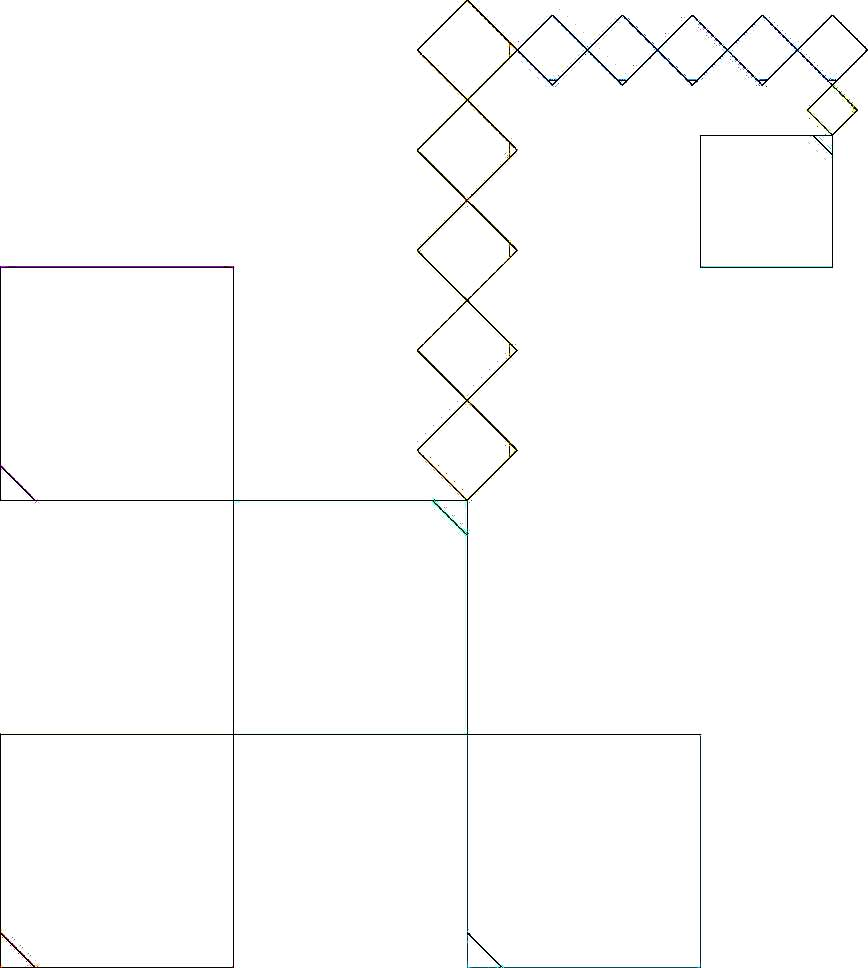
\includegraphics[width=.48\textwidth]{pl.jpg}\quad
        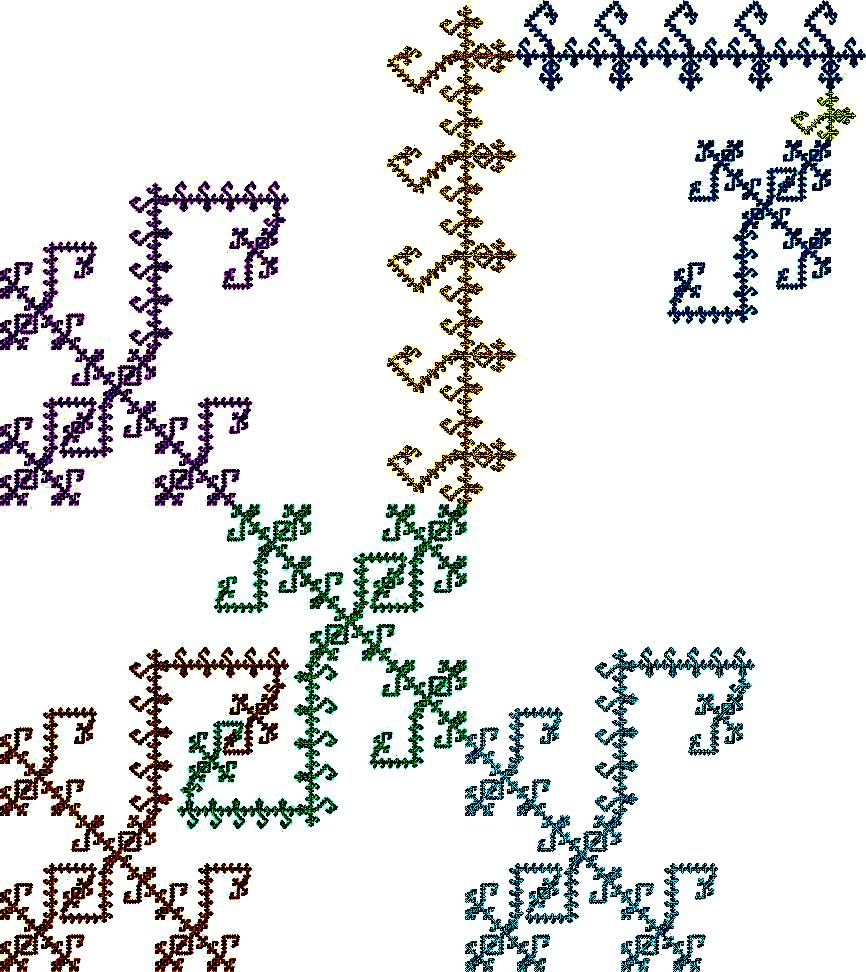
\includegraphics[width=.48\textwidth]{kl.jpg}}; 
    \draw (0.03,0.03)node{$B$} (0.61,0.61)node{$A$} (0.73,0.73)node{$B'$};
    \filldraw[fill=red] (0,0)circle(.007) (0.64,0.64)circle(.007) (0.76,0.76)circle(.007);
\end{tikzpicture}
\caption{$\al=-\pi$}% подпись к рисунку
\label{cntrex}% метка рисунка для ссылки на него  \ref{cntrex}
\end{figure}

\newpage

\begin{figure}[h!]
\centering
\begin{tikzpicture}[line cap=round,line join=round,>=stealth,x=10.0cm,y=10.0cm]
    \node[anchor=south west,inner sep=0] at (0,0) {
        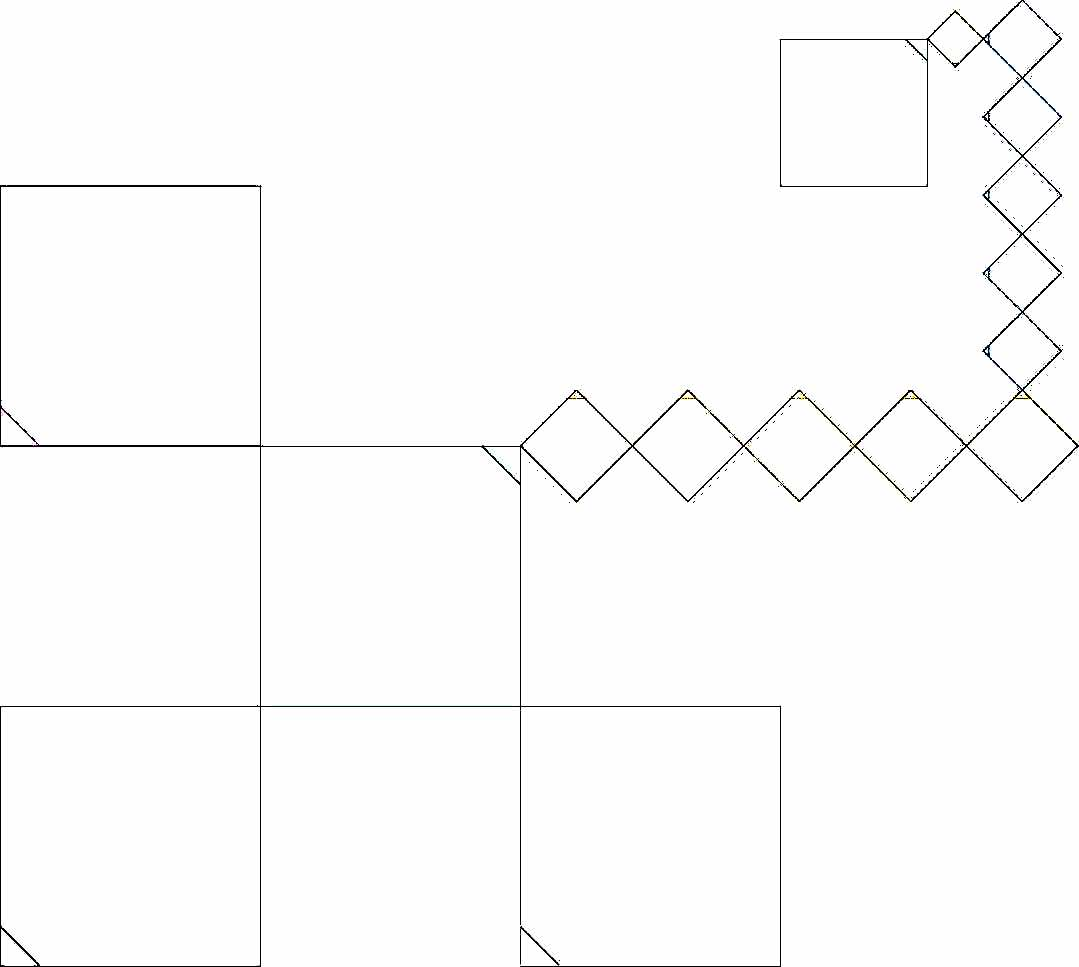
\includegraphics[width=.48\textwidth]{pr.jpg}\quad  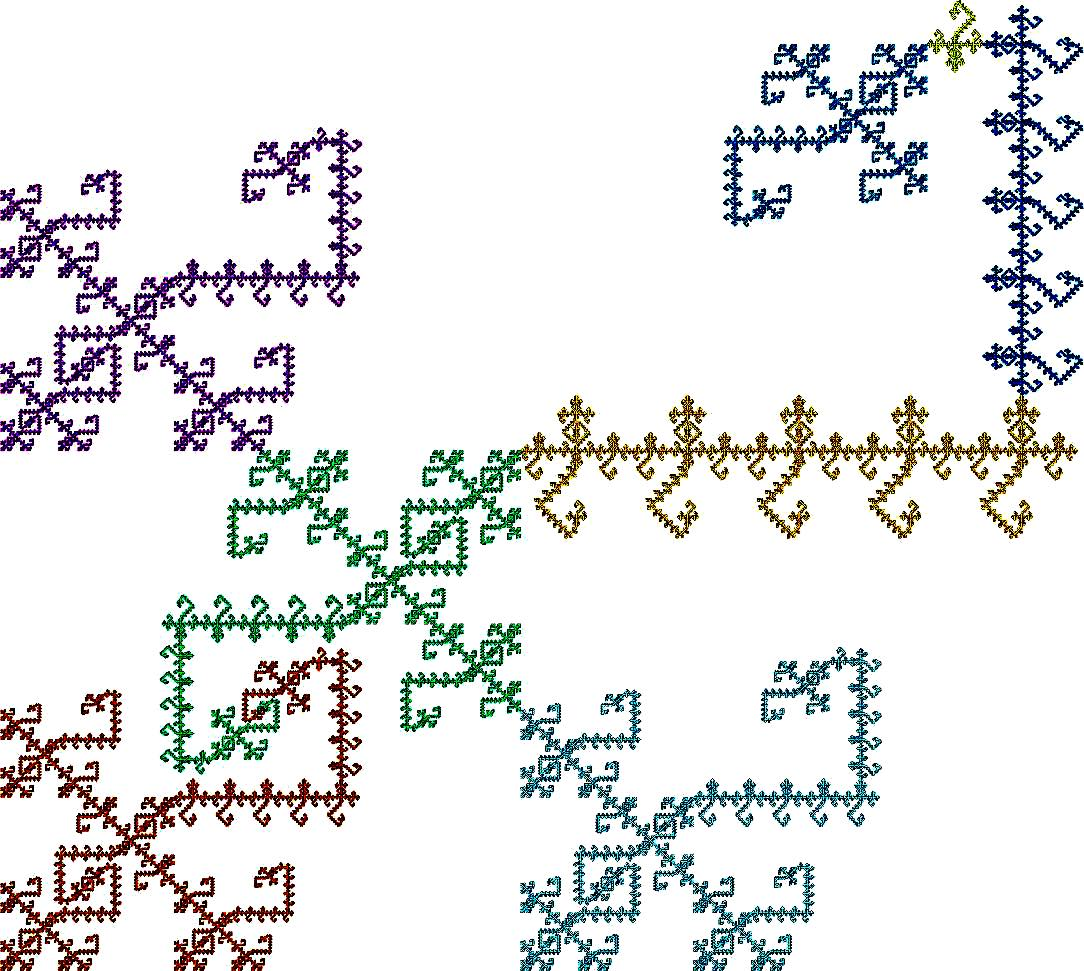
\includegraphics[width=.48\textwidth]{kr.jpg}}; 
    \draw (0.03,0.03)node{$B$} (0.55,0.55)node{$A$} (0.65,0.65)node{$B'$};
    \filldraw[fill=red] (0,0)circle(.007) (0.575,0.575)circle(.007) (0.68,0.68)circle(.007);
\end{tikzpicture}
\caption{$\al=\pi$}% подпись к рисунку
\label{cntrex}% метка рисунка для ссылки на него  \ref{cntrex}
\end{figure}

\begin{figure}[h!]
\centering
\begin{tikzpicture}[line cap=round,line join=round,>=stealth,x=10.0cm,y=10.0cm]
    \node[anchor=south west,inner sep=0] at (0,0) {
        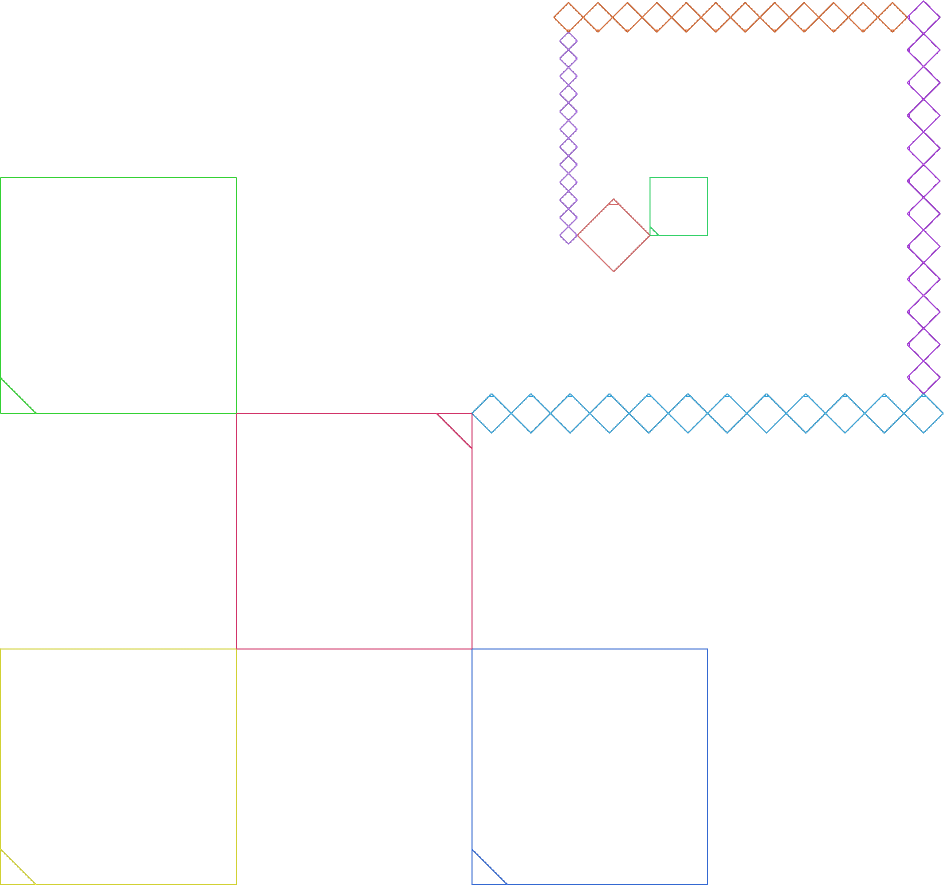
\includegraphics[width=.48\textwidth]{superd1.png}\quad  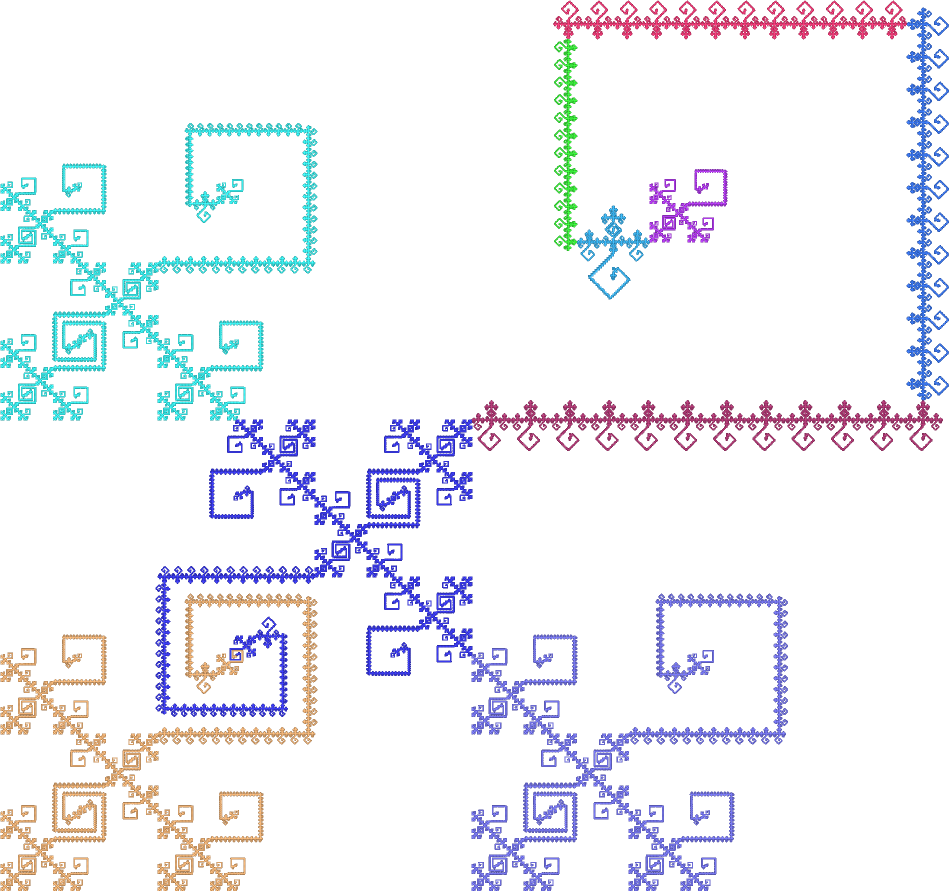
\includegraphics[width=.48\textwidth]{superd.png}}; 
    \draw (0.03,0.03)node{$B$} (0.62,0.62)node{$A$} (0.55,0.52)node{$B'$};
    \filldraw[fill=red] (0,0)circle(.007) (0.59,0.59)circle(.007) (0.55,0.55)circle(.007);
\end{tikzpicture}
\caption{$\al=2\pi$}% подпись к рисунку
\label{cntrex}% метка рисунка для ссылки на него  \ref{cntrex}
\end{figure}

\begin{definition}
Число $\lambda_A=\dfrac{\al}{\ln{r}}$ называется параметром циклической вершины $A$.
\end{definition}

\begin{definition}
Обобщенная $P$-полигональная система $\eS$ подобий удовлетворяет {\em условию совпадения параметров}, если для любого $B \in\cup_{i=1}^m  \eV_{P_i}$ и для любых циклических вершин $A,A'$  таких, что для некоторых $\bi,\bj\in I^*$,  $S_\bi(A)=S_\bj(A')=B$, выполняется равенство $\lambda _{A}=\lambda _{A'}$.
\end{definition}

Из Предложений \ref{1ordcyc} и \ref{fixparc}, и Леммы В.В.Ассеева о непересекающихся периодических дугах \cite[Lemma 3.1]{ATK} мы приходим к следующей Теореме о совпадении параметров:

\begin{theorem}\label{PMT}
Пусть обобщенная $P'$-полигональная система $\eS'$ является  $\da$-деформацией стягиваемой $P$-полигональной системы  $\eS$, а аттрактор $K'$ системы $\eS'$ является дендритом. Тогда система $\eS'$ Удовлетворяет условию совпадения параметров.
\end{theorem}

\dok Пусть $\eS$ -- обобщенная полигональная система, аттрактор $K$ которой -- дендрит. Пусть $C \in\cup_{i=1}^m  \eV_{P_i}$ и $A,A'\in \eV_P$ -- такие циклические вершины, что для некоторых $i,j\in I$  $S_i(A)=S_j(A')=C$. Обозначим образы $S_i(K)$ и $S_j(K)$ как $K_i,\ K_j$ соответственно. Без потери общности можно допустить, что точка $C$ имеет координату $0$ в $\bbc$. Поскольку для некоторых $\bi,\bj\in I^*$, $S_\bi(A)=A$ и $S_\bj(A')=A'$, отображения $S_{b1}=S_iS_\bi S_i^{-1}$ и $S_{b2}=S_jS_\bj S_j^{-1}$ имеют $C$  в качестве своей неподвижной точки, а $S_{b1}(K_i)\IN K_i$ и $S_{b2}(K_j)\IN K_j$. Пусть $S_{b1}(z)=q_\bi e^{i\al_\bi}z$ и $S_{b2}(z)=q_\bj e^{i\al_\bj}z$. Так параметрами вершин $A$ и $A'$ будут $\la_1=\dfrac{\al_\bi}{\log q_\bi}$ и  $\la_2=\dfrac{\al_\bj}{\log q_\bj}$. Пусть $\ga_{AB}\IN K$ и $\ga_{A'B'}\IN K$ являются инвариантными дугами для вершин $A$ и $A'$. Пусть также  $\ga_1=S_i(\ga_{AB})$ и $\ga_2=S_j(\ga_{A'B'})$. Тогда $S_{b1}(\ga_1)\IN \ga_1$ и $S_{b2}(\ga_2)\IN \ga_2$. По Лемме В.В.Ассеева о непересекающихся периодических дугах \cite[Lemma 3.1]{ATK} следует, что если $\ga_1\cap\ga_2=\{C\}$, то $\la_1=\la_2$.\vse\\

Для проверки условия совпадения параметров в полигональной системе очень удобно использовать индексные диаграммы.

\begin{definition}\label{diagram}
Пусть $\eS=\{S_1,\ldots,S_m\}$ -- обобщенная $P$-полигональная система, аттрактор $K$ которой -- дендрит. Пусть $\eV=\{v_1,\ldots,v_n\}$ -- множество вершин многоугольника $P$. Индексной диаграммой мы назовем ориентированный граф $D=(\eV,E)$, для которого дуга $(v_i,v_j)\in E$ тогда и только тогда, когда существует такое $S_k\in\eS$, что $v_i=S_k(v_j)$. 
\end{definition}

Индексные диаграммы и в самом деле довольно удобны в использовании, ведь они позволяют наглядно посмотреть на то, какие вершины каким подчинены и какие вершины являются циклическими какого-либо порядка. Поскольку у вершин, находящимся в одном цикле индексной диаграммы или же подчиненным такому циклу, совпадают параметры, то это является большим подспорьем при проектировании обобщенных полигональных систем. В противном случае, если не пользоваться этим свойством циклических вершин, то остается только подгонять размеры и повороты подобий так, чтобы их параметры совпадали.

\begin{figure}[h!]
\begin{center}
\begin{minipage}[h]{0.45\linewidth}
\begin{tikzpicture}[line cap=round,line join=round,>=stealth, scale=1]\scriptsize
\node  at (0,0) {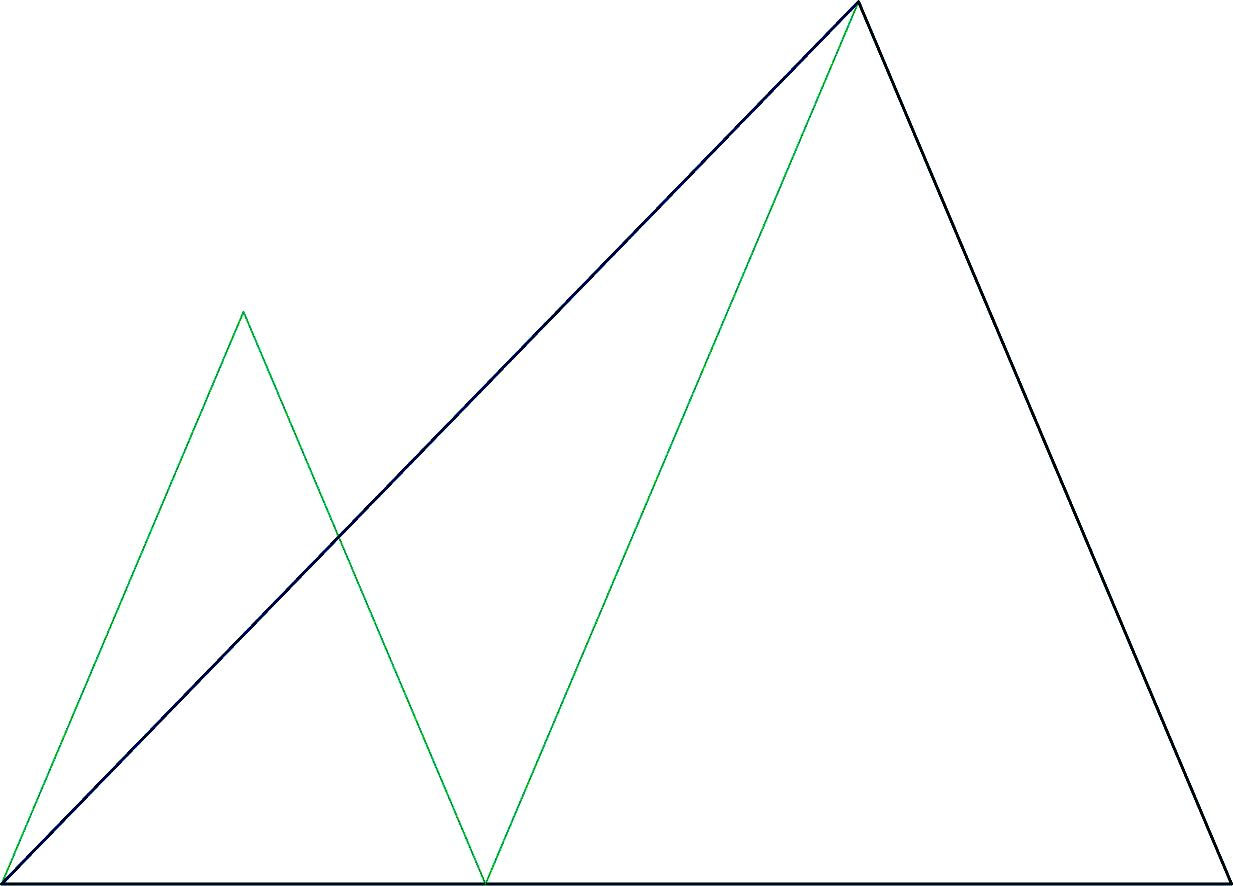
\includegraphics[width=1\textwidth]{gps1.jpg} };
\node at(-4,-2.6){1};
\node at(4,-2.5){2};
\node at(1.5,3){3};
\end{tikzpicture}
\caption{Нумерация вершин}% подпись к рисунку
\label{logimg0}% метка рисунка для ссылки на него  \ref{logimg0}
\end{minipage}
\hfill
\begin{minipage}[h]{0.45\linewidth}
\vspace{2.5cm}
\hspace{1cm}
\begin{tikzpicture}[line cap=round,line join=round,>=stealth, scale=1]\scriptsize
\node[shape=circle,draw, shift={( 0,0)}] (a1) {1};
\node[shape=circle,draw, shift={( 4,0)}] (a2) {2};
\node[shape=circle,draw, shift={( 2,3)}] (a3) {3};
\path[->,>={Latex[length=5pt]}] 
    (a1) edge (a2)
    (a2) edge (a3)
    (a3) edge (a1);
\end{tikzpicture}
\caption{Индексная диаграмма}% подпись к рисунку
\label{logimg1}% метка рисунка для ссылки на него  \ref{logimg1}
\end{minipage}
\end{center}
\end{figure}

Технически, теорема о совпадении параметров показывает необходимое условие того, что аттрактор $\da$-деформации будет дендритом. Однако если стягиваемую полигональную систему деформировать слишком сильно, то даже при соблюдении условия совпадения параметров аттрактор $\da$-деформации и не быть дендритом. Значит нам нужны ограничения при деформациях. Поэтому далее мы оценим $\da$ в доказательстве теоремы о малых деформациях. Эта оценка и будет представлять из себя достаточное условие того, что аттрактор $\da$-деформации будет дендритом.



\subsection{Основные параметры стягиваемой полигональной системы}

Для любого множества $X\IN\rr^2$ или точки $A$ через $V_\ep(X)$ (соотв.$V_\ep(A)$) мы обозначаем $\ep$-окрестности множества $X$ (соотв. точки $A$) на плоскости.\\

$\bm{\rho_0:}$  Возьмем такое $\rho_0>0$, что:\\ 
(i) для любой вершины $A\in \eV_P$,   $V_\rho(A) \bigcap P_k \ne \0 \Rightarrow A\in P_k$;\\ 
(ii) для любых $x, y \in P$, для которых существуют такие $P_k, P_l$, что $x \in P_k, y \in P_l$ и $P_k \bigcap P_l = \0$, выполняется $d (x, y) \ge \rho_0$. \\ 

\begin{figure}[h!]
\centering
\begin{tikzpicture}[line cap=round,line join=round,>=stealth ,scale=1]\scriptsize
\node at (-6.3,-2) {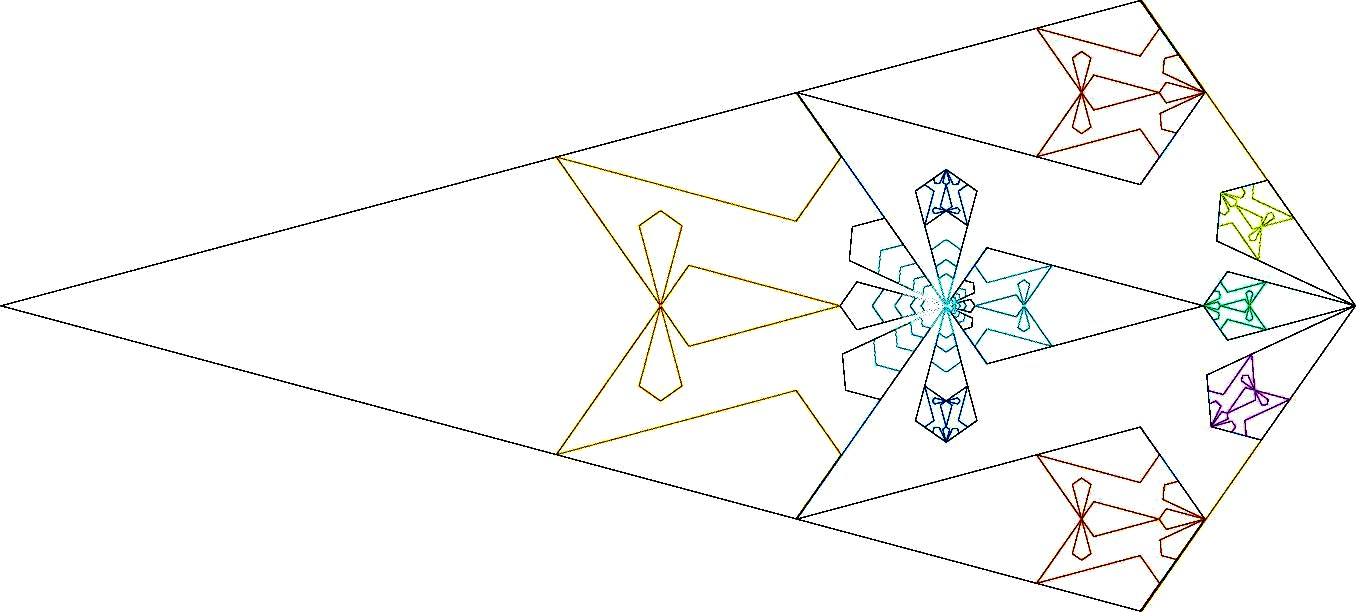
\includegraphics[width=.57\textwidth]{Pol2a.jpg}};
\node at (2,-2.68) {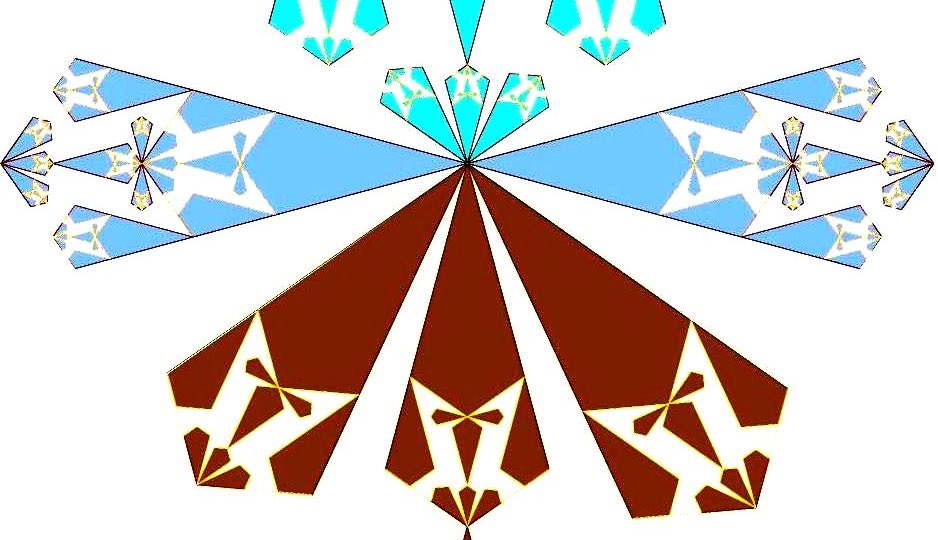
\includegraphics[width=.35\textwidth]{1111.jpg}};
%\draw[step=.1,lightgray,ultra thin] (-11,-5) grid (5,0);
  %\draw[step=.2,yellow,ultra thin] (-11,-5) grid (6,0);
  % \draw[step=1,green, thin] (-11,-5) grid (5,0);
  	  \path[thick,red] (2,-2) edge[->]  (4.7,-3.2);
	  \path[thin,red] (-1.46,-2) edge[]  (-2.8,-2.62);
	  \path[thin,red] (-1.46,-2) edge[]  (-2.9,-2.39);
	    %\draw (2,-2) circle [radius=2.95];
	    \draw[thick,red] (4.1,-4.1) arc (-45:20:2.96);
	     \draw[thick,red] (-.1,-4.1) arc (-135:-200:2.96);
	     \draw[thin,red] (-2.55,-2.5) arc  (-155:-165.5:1.08);
	    \draw [thick,blue](2,-2) circle [radius=.35];
	    \draw [thick,red](-4.38,-2) circle [radius=0.98];
	    \draw [thin,blue](-4.38,-2) circle [radius=0.12];
	    \node at(4.4,-3.3){$\bm\rho_2$};\node at(1.5,-2.2){$\bm\rho_1$};\node at(-2.8,-2.5){$\bm\al_0$};
\end{tikzpicture}
\caption{Выбор параметров $\al_0$, $\rho_1$ и $\rho_2$ для полигональной системы.}% подпись к рисунку
\label{param}% метка рисунка для ссылки на него  \ref{param}
\end{figure}

$\bm{\rho_1,\rho_2:}$    Из теоремы \ref{refsys} следует, что для любой вершины $B\in \eV_\wP$  существует конечное множество циклических вершин $A_{i_1},...,A_{i_k}\in \eV_P$ и мультииндексов $\bj_1,...,\bj_k$  таких, что для любого $l=1,...,k$ справедливо $S_{\bj_l}(A_l)=B$  и $S_{i_l}(A_l)=A_l$, а множество $\bigcup\limits_{l=1}^k S_{\bj_l}S_{i_l}^n(K)$ является окрестностью точки $B$ в $K$ для любого $n\ge 0$.\\
Пусть $\rho_1$ и $\rho_2$ являются такими положительными числами, что для любой  вершины $B\in \eV_\wP$ 
\beq\label{ro12} (V_{\rho_1}(B)\cap K)\IN \bigcup\limits_{l=1}^k S_{\bj_l}(P_{i_l})\mbox{\qquad   and  \qquad  }
\bigcup\limits_{l=1}^k P_{\bj_l}\IN V_{\rho_2}(B).\eeq
  
$\bm{\al_0:}$  Пусть $\al_0$ обозначает минимальный угол между теми сторонами многоугольников $P_i, P_j, i,j\in I$, которые имеют общую вершину.
  
{\bf Расположение отображений, фиксирующих циклические вершины.} Пусть $\eS$ --- это стягиваемая $P$-полигональная система, все циклические вершины которой имеют порядок 1. 
В этом случае мы можем упорядочить индексы в $I$ и пронумеровать вершины в $\eV_P$ таким образом, что каждая циклическая $A_l$ будет фиксированной точкой отображения $S_l\in \eS$. 
Заметим, что $S_l$ --- это гомотетии $S_l(z)=q_l(z-A_l)+A_l$, многоугольник $P$  лежит внутри угла $\Om(P, A_l)$ и $K\mmm \{A_l\} =\bigsqcup\limits_{n=0}^\8S_l^n(K\mmm K_l)$. 
Число точек в $\overline{K_l\mmm S_l(K_l)}\cap S_l(K_l)$  конечно и равно порядку ветвления точки $A_l$ в $K$.



\subsection{Теорема о малых деформациях}

{\bf Некоторые допущения.} Отныне мы будем использовать следующее соглашение: $\eS=\{S_1,...,S_m\}$ будет обозначать стягиваемую $P$-полигональную систему, а $\eS'=\{S'_1,...,S'_m\}$ -- обобщенную $P'$-полигональную систему, являющуюся задаваемой отображением $f$ $\da$-деформацией системы $\eS$.\\ Для любого $k\in I$, $S_k(z)=q_k e^{i\al_k}(z-z_k)+z_k$ и $S'_k(z)=q'_k e^{i\al'_k}(z-z'_k)+z'_k$, где $z_k=\fix(S_k)$. Мы также по умолчанию предполагаем, что $\diam P=1$. Мы предполагаем, что \beq\label{assum}\da<q_{min}/8\mbox{\quad and \quad}\da<(1-q_{max})/8\eeq

\begin{lemma}\label{lasin}
Пусть  $\eS'=\{S'_1,...,S'_m\}$ -- это  $\da$-деформация стягиваемой $P$-полигональной системы $\eS$. Для достаточно малого $\da$ и для любого $k\in I$
\beq\label{asin} \dfrac{q_k-2\da}{1+2\da}\le q'_k\le \dfrac{q_k+2\da}{1-2\da}  \mbox{\quad \rm и  \quad}|\al_k'-\al_k|\le \arcsin 2\da+\arcsin \dfrac{2\da}{q_k}.\eeq
\end{lemma} 
\dok 
Пусть $A,B$ -- это такие вершины многоугольника $P$, что $|B-A|=1$. Запишем $S_k(A)=A_k$ и $f(A)=A'$, и, используя аналогичные обозначения для всех вершин, определим $S'_k(A')=A'_k=f(A_k)$. Заметим, что $\dfrac{B_k-A_k}{B-A}=q_k e^{i\al_k}$ и $\dfrac{B'_k-A'_k}{B'-A'}=q'_k e^{i\al'_k}$.

Поскольку отображение $f$ сдвигает $A,B,A_k,B_k$ на расстояние $\le\da$, то   $|(B-A)-(B'-A')|\le 2\da$ и $|(B_k-A_k)-(B'_k-A'_k)|\le 2\da$.
Следовательно, $|(B_k-A_k)|-2\da\le|(B'_k-A'_k)|\le |(B_k-A_k)|+2\da$ и
\beq\label{dal}\al'_i-\al_i=\arg\dfrac{B'_k-A_k'}{B'-A'}\dfrac{B-A}{B_k-A_k}=\arg\dfrac{B'_k-A_k'}{B_k-A_k}-\arg\dfrac{B'-A'}{B-A}\eeq
Это влечет неравенство (\ref{asin}).  \vse\medskip

В соответствии с допущениями (\ref{assum}), 
\beq 3q_{min}/5<\dfrac{q_{min}-2\da}{1+2\da}<q'_k<\dfrac{q_{max}+2\da}{1-2\da}<\dfrac{1+3q_{max}}{3+q_{max}};\eeq\\ 
принимая во внимание то, что $q_k<1$ и $1-2\da>3/4$, и что если $0<x<.5$, то $\arcsin x<1.05x$, мы получаем
 \beq\label{dadq}\Da q_k=|q'_k-q_k|<\dfrac{2\da(1+q_k)}{1-2\da}<6\da  \mbox{\quad и \quad} \Da \al_k=|\al'_k-\al_k|< 
C_\al\da ,\eeq где $C_\al=2.1(1+1/q_{min})$.\smallskip\\

Пусть $V_\da(P)$ обозначает $\da$-окрестность многоугольника $P$.

\begin{lemma}
Пусть  $\eS'=\{S'_1,...,S'_m\}$ будет  $\da$-деформацией стягиваемой $P$-полигональной системы $\eS$. Множество $U=V_{\da_1}(P)$, где $\da_1=\dfrac{8\da}{1+3q_{max}}$, удовлетворяет условию
\beq \label{vda1}\mbox{\rm  для любого  } k\in I,\ \ \ \    S_k(U)\IN U\mbox{\quad\rm и \quad}S'_k(U)\IN U\eeq
\end{lemma} 

\dok
По Определению \ref{deform}, $V_\da(P_k)\NI P'_k$, $V_\da(P'_k)\NI P_k$, и поскольку вершины многоугольника $P$ также перемещаются на расстояние меньше чем $\da$,
$V_\da(P)\NI P'$ и $V_\da(P')\NI P$.

Таким образом, мы можем написать $S_k'(P')\IN V_\da(P_k)\IN V_\da(P)$ из чего следует, что
$S_k'(P)\IN V_{2\da}(P_k)\IN V_{2\da}(P)$.\\ Для любого положительного $\rho$ мы имеем включение $S_k'(V_\rho(P))\IN V_{2\da+q'_k\rho}(P)$. В случае, когда $\rho= 2\da+q'_k\rho$ это влечет за собой $S_k'(V_{\rho}(P))\IN V_{\rho}(P)$, где $\rho=\dfrac{2\da}{1-q_k'}$. Поскольку $q_k'\le 
q_k+2\da$, $q'_{max}\le q_{max} +2\da<\dfrac{3q_{max}+1}{4}$, мы приходим к включениям (\ref{vda1}).\vse

\begin{lemma}
Для любого $z\in V_{\da_1}(P)$, $|S'_k(z)-S_k(z)|<C_\Da\da$, где $C_\Da=14+2C_\al$.
\end{lemma}

\dok Возьмем $z\in V_{\da_1}(P)$ и оценим разность $S'_k(z)-S_k(z)$. Её можно представить в виде $S'_k(A)-S_k(A)+(q'_ke^{i\al'_k}-q_ke^{i\al_k})(z-A)$. Поэтому \beq\label{delta}|S'_k(z)-S_k(z)|<|S'_k(A)-S_k(A)|+(|q'_k-q_k|+q_k|e^{i\al'_k}-e^{i\al_k}|)|z-A|.\eeq 
Ввиду $|z-A|<1+\da_1<2$ и $|S'_k(A)-S_k(A)|<2\da$, правая часть неравенства (\ref{delta}) не превышает $2\da+2(6\da+C_\al\da)$.\vse

\begin{prop}\label{deltaK}
Пусть $\pi:I^\8\to K$ и $\pi':I^\8\to K'$ -- индексные отображения для систем $\eS$ и $\eS'$ соответственно.\\
1. Согласно предположениям (\ref{assum}), для любого $\sa\in I^\8$, 
\beq\label{dKeq} |\pi'(\sa)-\pi(\sa)|< C_K\da \mbox{   где   }C_K=\dfrac{2C_\Da}{1-q_{max}}\eeq 
2. Для любого $n$, если система $\eS^{'(n)}$ является обобщенной полигональной системой, то это  $C_K\da$-деформация системы $\eS^{(n)}$.
\vse
\end{prop}

\begin{rmk}\label{Sshift}
Пусть  $\eS'=\{S'_1,...,S'_m\}$ --- это  $\da$-деформация стягиваемой $P$-полигональной системы $\eS$. Пусть $A\in S_j(\eV_P)$ для некоторого $j\in I$. Пусть $g(z)=z-A+A'$ и $\hat S''_k=g\circ S'_k\circ g^{-1}$.
Тогда $\eS''=\{S''_1,...,S''_m\}$ является $2\da$-деформацией системы $\eS$, для которой $A''=A$, $K''=g(K')$, $P''_\bj=g(P_\bj)$. Поскольку $g$ -- это сдвиг, оценки (\ref{asin}) и (\ref{dadq}) для $\eS''$ остаются неизменными с тем же $\da$, в то время как $|\pi''(\sa)-\pi(\sa)|< (C_K+1)\da$. Таким образом мы обозначаем  $\da_2=(C_K+1)\da$. \end{rmk}

Принимая во внимание Предложения \ref{1ordcyc}и \ref{deltaK}, достаточно доказать теорему для случая, когда все циклические вершины системы $\eS$ имеют порядок 1.

\begin{prop}
Пусть $P'$-полигональная система $\eS'$ является $\da$-деформацией стягиваемой $P$-полигональной системы $\eS$. Пусть $A\in \eV_P$ -- циклическая вершина (порядка 1) и $S_k(z)=q_ke^{i\al_k}(z-A)+A$.  Тогда угол поворота $\al_k$ отображения $S'_k$ отображения  $S'_k$  удовлетворяет неравенству \begin{equation}\label{parmeq}|\la_k|\le\dfrac{\arcsin 2\da+\arcsin\dfrac{2\da}{q_k}}{|\log(q_k+2\da)-\log(1-2\da)|}\end{equation}
\end{prop}

\dok Формула (\ref{parmeq}) следует непосредственно из Леммы \ref{lasin}.\vse\\

При допущениях (\ref{assum}) справедливо неравенство \beq\label{prmeq2}|\la_k|<C_\la\da\mbox{, где }C_\la=\dfrac{2.1(1+1/q_{max})}{\log(3+q_{max})-\log(3q_{max}+1)}.\eeq

  
\begin{lemma}
Пусть $\eS$ -- стягиваемая $P$-полигональная система, циклические вершины котрой имеют порядок 1, а $\eS'$ -- её $\da$-деформация. Тогда если \beq \label{mineq}2.1\dfrac{\da_2}{\rho_1}+\la\log\dfrac{\rho_2+\da_2}{\rho_1-\da_2}<\al_0 \mbox{ и }  2\da_2<\rho_0,\eeq то система $\eS'$ удовлетворяет Условию (\ref{icnd})
\end{lemma}  
  

\dok  Возьмем вершину $B\in V_\wP$. Для удобства мы можем предположить, что $B=0$, и, Следуя Замечанию \ref{Sshift}, мы также можем предположить, что отображение $f$ фиксирует вершину $B=0$, поэтому $B'=B=0$.   Пусть $W_l=S_{\bj_l}(K\mmm K_{i_l})$. Отображения $\bar S_l=S_{\bj_l}S_{i_l}S_{\bj_l}^{-1}$ являются гомотоетиями с такой фиксированной точкой $B$, что 
\beq\label{kbj} K_{\bj_l}\mmm\{B\}=\bigsqcup\limits_{n=0}^\8\bar S_l^n(W_l)\eeq 
Аналогично, пусть $W'_l=\hat f(W_l)$ и $\bar S'_l=S'_{\bj_l}S'_{i_l}S_{\bj_l}^{'-1}$. Тогда
 \beq \label{kpbj} K'_{\bj_l}\mmm\{B\}=\bigsqcup\limits_{n=0}^\8\bar S_l^{'n}(W'_l)\eeq
Заметим, что  $\bar S_l(z)=q_{i_l}z$ и $\bar S'_l(z)=q'_{i_l}e^{i\al_{i_l}}z$ для любого $l$, а из за условия совпадения параметров существует такой  $\la$, что для любого $l$ $\al_{i_l}=\la\log q'_{i_l}$. 
  
Рассмотрим отображение $z = exp(w)$ плоскости $(w = \ro+i\fy)$ как универсальное покрытие проколотой плоскости $\bbc\mmm\{0\}$. 

Рассмотрим многоугольники $P_{\bj_l}$ и выберем свои поднятия на плоскости $(w = \ro+i\fy)$.
Мы можем предположить, что эти поднятия лежат в соответствующих горизонтальных полосах $\te^-_l\le\fy\le\te^+_l$, где $0<\te^-_l<\te^+_l<2\pi$ и $\te^+_l+\al_0<\te^-_{l+1}$ для любого $l<k$, и $\te^+_k+\al_0<\te^-_1 +2\pi$.
Мы также рассматриваем поднятия множеств $K_{\bj_l}$, $W_l$, $K'_{\bj_l}$ и
$W'_l$. Обозначим эти поднятия как $\eK_{\bj_l}$, $\eW_l$, $\eK'_{\bj_l}$ и
$\eW'_l$.
Из уравнений \ref{kbj} и \ref{kpbj} следует, что
\beq\label{ekbj} \eK_{\bj_l}=\bigsqcup\limits_{n=0}^\8\bar T_l^n(\eW_l) \mbox{\quad и \quad} \eK'_{\bj_l}=\bigsqcup\limits_{n=0}^\8\bar T_l^{'n}(\eW'_l), \eeq  
где $T_l(w)=w+\log q_l$   и   $T'_l(w)=w+(1+i\la)\log q'_l$ являются параллельными сдвигами, для которых$T_l(\eK_l)\IN \eK_l$ and $T'_l(\eK'_l)\IN \eK'_l$.

\begin{figure}[h!]
\begin{center}
\begin{minipage}[h]{0.42\linewidth}
\begin{tikzpicture}[line cap=round,line join=round,>=stealth ,scale=1]\scriptsize
\node at (0,0) {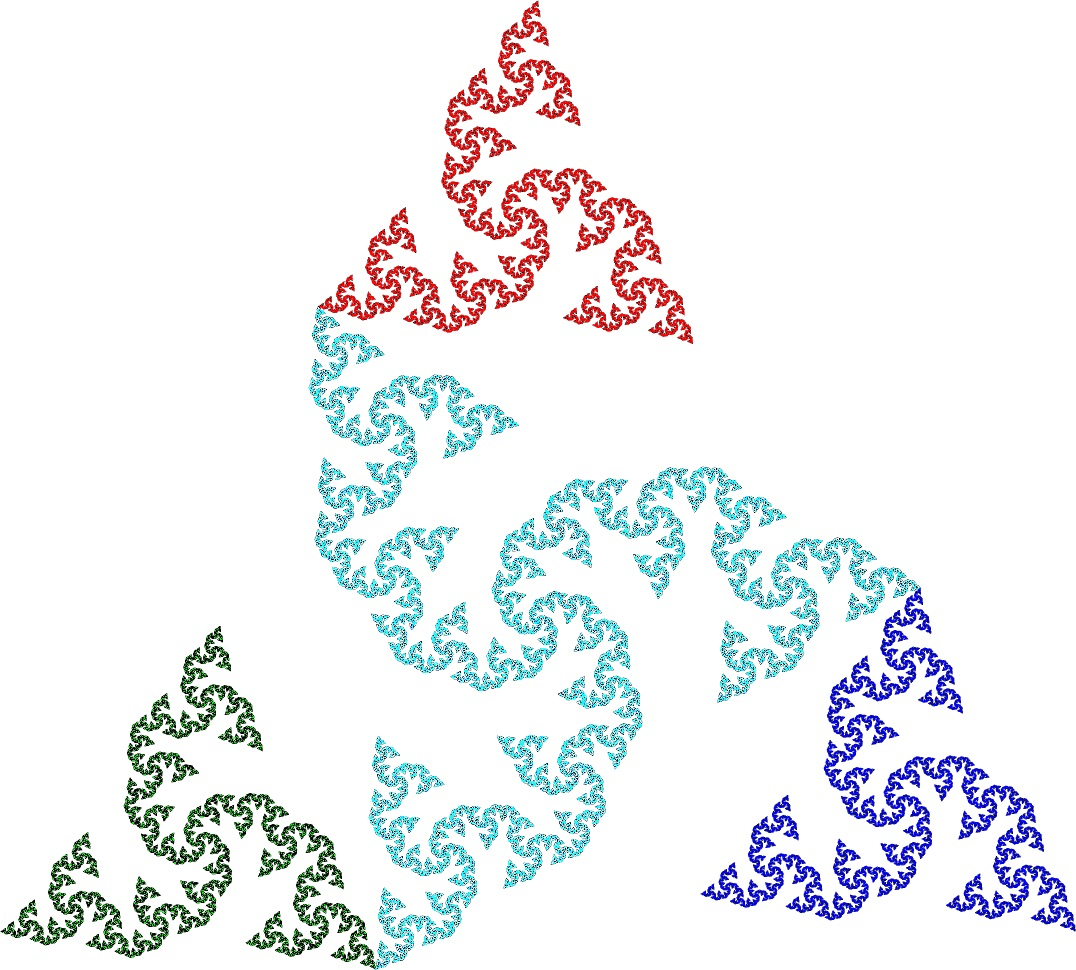
\includegraphics[width=1\textwidth]{dirimage.jpg}};
\node at(-1,-2.6){$B$};
\node at(0,-0.5){$O$};
\filldraw[fill=red] (-1,-3.1)circle(.07) (0,-0.95)circle(.07);
\end{tikzpicture}
\caption{Изображение множества $K'$}% подпись к рисунку
\label{logimg0}% метка рисунка для ссылки на него  \ref{logimg0}
\end{minipage}
\hfill
\begin{minipage}[h]{0.55\linewidth}
\vspace{1.7cm}
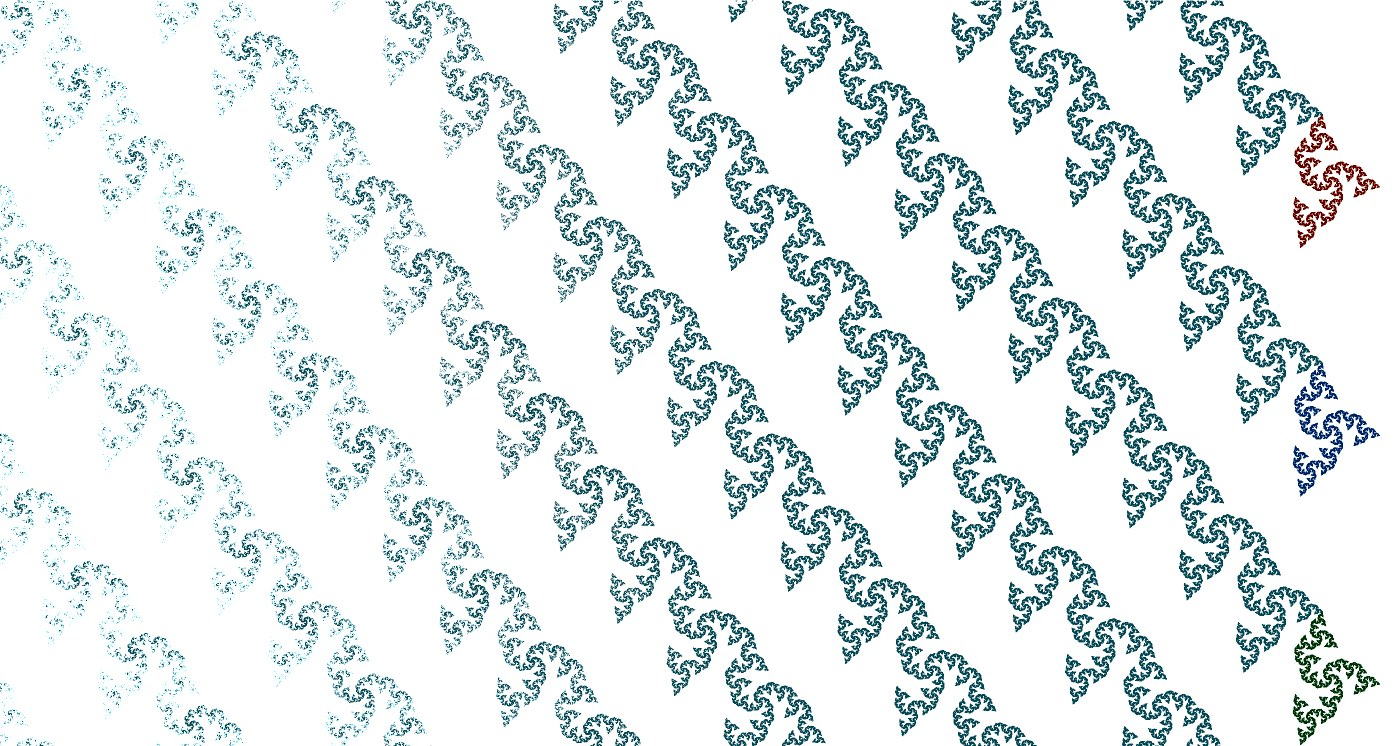
\includegraphics[width=1\textwidth]{logimage3.jpg}
\caption{$K'$ после отображения $w=\log(z-O)$}% подпись к рисунку
\label{logimg1}% метка рисунка для ссылки на него  \ref{logimg1}
\end{minipage}
\end{center}
\end{figure}


\begin{figure}[h!]
\centering
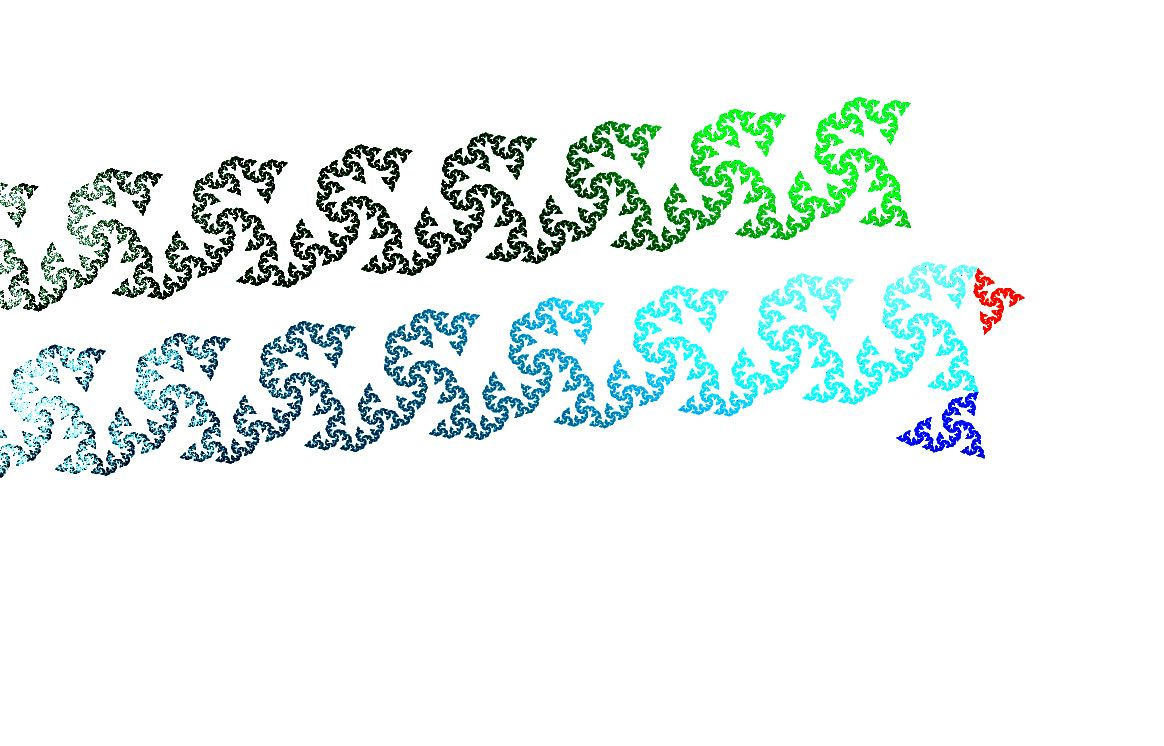
\includegraphics[width=0.9\textwidth]{logimage2.jpg}
\caption{$K'$ после отображения  $w=\log(z-B)$.}% подпись к рисунку
\label{logimg2}% метка рисунка для ссылки на него  \ref{logimg2}
\end{figure}

Множества $\eK_l$ лежат в полуполосах $ \ro\le \log\rho_2, \te^-_l\le\fy\le\te^+_l$, в то время как множества $\eW_l$ содержатся в прямоугольниках $R_l=\{\log\rho_1 \le\ro\le \log\rho_2, \te^-_l\le\fy\le\te^+_l\}$.

Тогда множества $\eW'_l$ лежат в прямоугольнике \beq R'_l=\left\{\log(\rho_1-\da_2)\le\ro\le \log(\rho_2+\da_2), \te^-_l-1.05\dfrac{\da_2}{\rho_1}\le\fy\le\te^+_l+1.05\dfrac{\da_2}{\rho_1}\right\}\eeq

Каждое объединение  $\bigcup\limits_{n=0}^\8T^{'n}_l(R'_l)$ лежит в полуполосе 
\beq \begin{cases}\ro\le \log(\rho_2+\da_2)\\   \te^-_l-1.05\dfrac{\da_2}{\rho_1}-\la \log(\rho_2+\da_2)\le\fy-\la\ro\le \te^+_l+1.05\dfrac{\da_2}{\rho_1}-\la \log(\rho_1-\da_2)\end{cases}\eeq

Поэтому множество $\eK'_{\bj_l}$ тоже лежит в этой полуполосе
Тогда если 
\beq\te^+_{l-1}+1.05\dfrac{\da_2}{\rho_1}-\la \log(\rho_1-\da_2)<\te^-_l-1.05\dfrac{\da_2}{\rho_1}-\la \log(\rho_2+\da_2),\eeq то $\eK'_{\bj_{l-1}}\cap\eK'_{\bj_l}=\0$.

Мы можем гарантировать, что такое неравенство справедливо для любого $l$, если 
$2.1\dfrac{\da_2}{\rho_1}+\la\log\dfrac{\rho_2+\da_2}{\rho_1-\da_2}<\al_0$.

Если, кроме того, $2\da_2<\rho_0$, то для любоых $i_1,i_2\in I$  таких что $P_{i_1}\cap P_{i_2}=\0$, $P'_{i_1}\cap P'_{i_2}=\0$  и $K'_{i_1}\cap K'_{i_2}=\0$ откуда следует условие (\ref{icnd}).
\vse
 
 
\begin{theorem}\label{mainthm}
Пусть $\eS$ -- стягиваемая $P$-полигональная система. Существует такое $\da>0$, что для любой $\da$-деформации $\eS'$ системы $\eS$, удовлетворяющей условию совпадения параметров, аттрактор $K(\eS')$ будет дендритом, гомеоморфным $K(\eS)$.
\end{theorem}

\dok  Пусть все циклические вершины $P$-полигональной системы $\eS$ имеют порядок 1. Если мы предположим, что $\da_2<\rho_1/4$, а $\da_2<(1-\rho_2)/4$, и скомбинируем неравенства \ref{dadq}, \ref{dKeq}, \ref{prmeq2}, \ref{mineq}, мы увидим, что, если выполняются следующие неравенства::\\
1.$\da<\dfrac{q_{min}}{8}$;\qquad  2. $\da<\dfrac{1-q_{max}}{8}$;\qquad  3. $\da<\dfrac{\rho_0}{2(C_K+1)}$;\qquad  4. $\da<\dfrac{\rho_1}{4(C_K+1)}$;\\
5. $\da<\dfrac{1-\rho_2}{4(C_K+1)}$; \qquad \qquad и \qquad  6. $\da<\dfrac{\al_0}{\dfrac{2.1(C_K+1)}{\rho_1}+C_\la\log\dfrac{1+3\rho_2}{3\rho_1}}$,\\ 
то аттрактор $K'$ $\da$-деформации $\eS'$ системы $\eS$ удовлетворяет условию (\ref{icnd}). Следовательно $K'$ -- дендрит. По Теореме \ref{attrmap}, отображение $\hat f:K\to K'$ биективно, и следовательно оно является гомеоморфизмом.
 
Предположим теперь, что $\eS$ имеет циклические вершины порядка больше 1, и пусть $M=12+4.2\left(1+\dfrac{1}{q_{min}}\right)$. Существует такое $n$, что система $\eS^{(n)}$ имеет циклические вершины порядка 1. Предположим, что любая $\da$-деформация системы $\eS^{(n)}$ порождает дендрит. Тогда для любой $\da/M$-деформации $\eS'$ системы $\eS$, система $\eS^{'(n)}$ будет $\da$-деформацией системы $\eS^{(n)}$.\vse


\newpage
\section{Некоторые примеры}


На рисунках \ref{ris43} и \ref{ris46} показаны деформации, в которыху первого параметры совпадают, но взята слишком большая $\delta$ для деформации. На рисунке же \ref{ris46}  $\delta$ взята достаточно малая, чтобы аттрактор на рисунке \ref{ris46} был дендритом.


\begin{figure}[h!]
\begin{center}
\begin{minipage}[h]{1\linewidth}
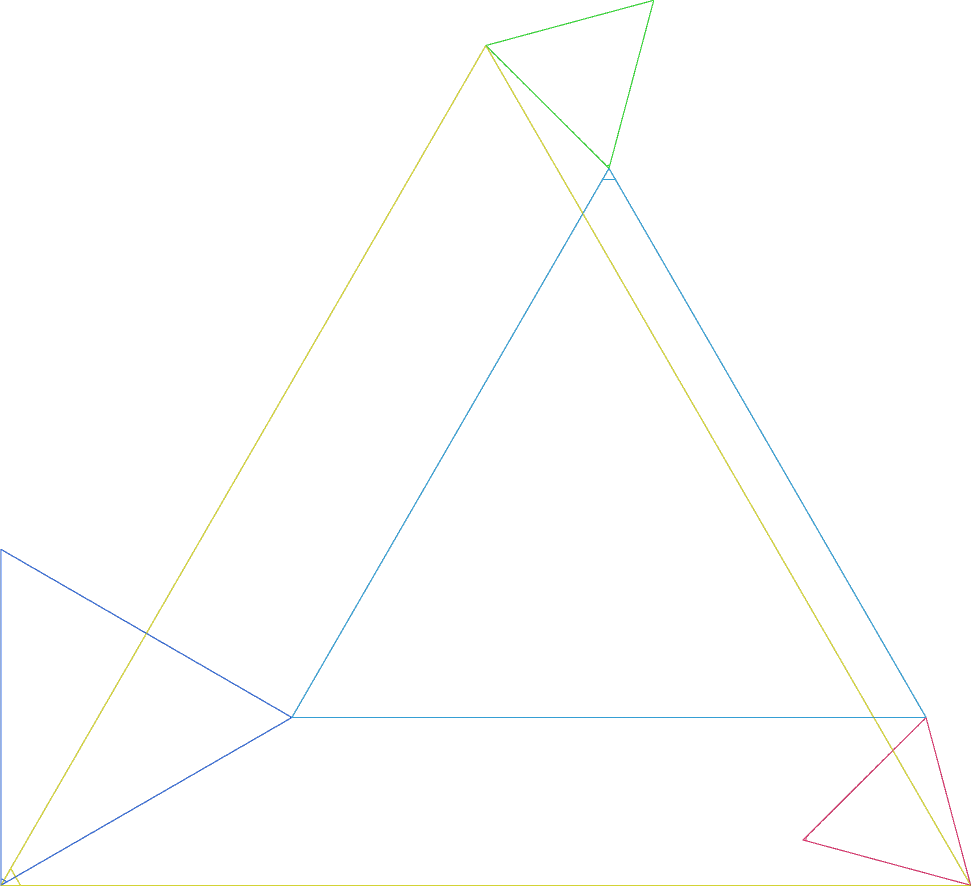
\includegraphics[width=0.45\linewidth]{231.png}
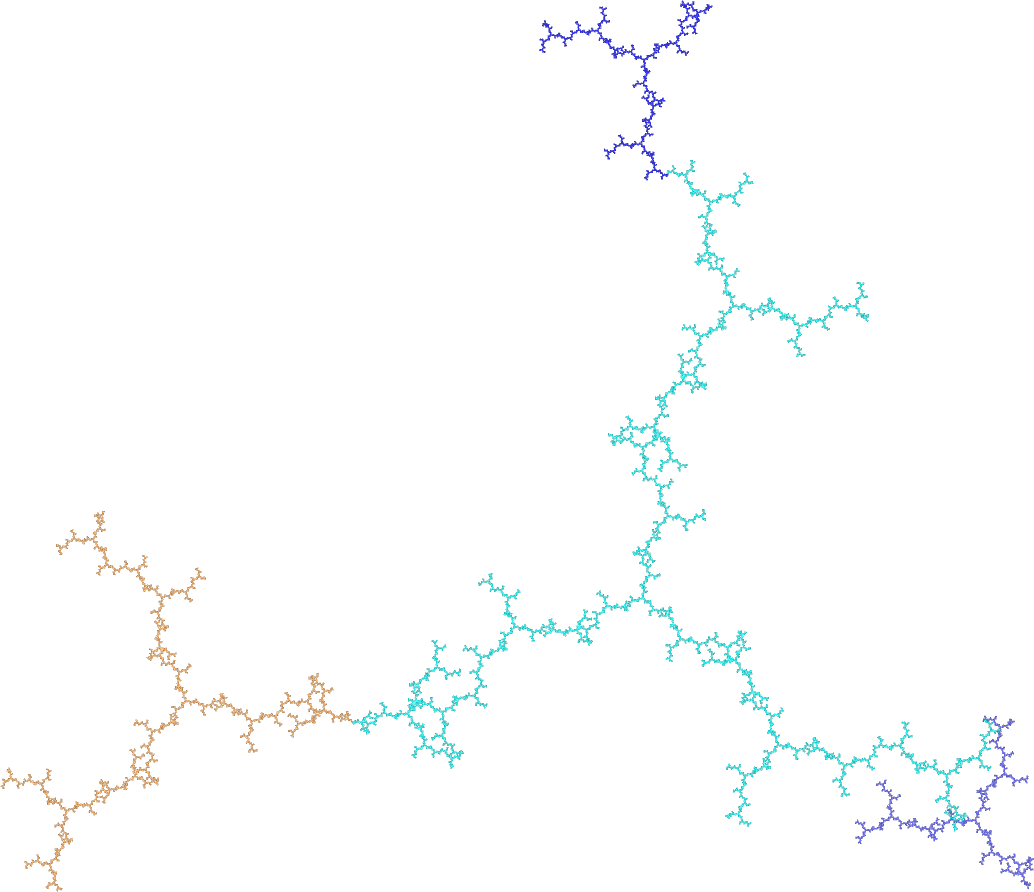
\includegraphics[width=0.45\linewidth]{232.png}
\caption{Не дендрит, параметры совпадают, но деформация большая } % подпись к рисунку
\label{ris43} % метка рисунка для ссылки на него  \ref{ris43}
\end{minipage}
\end{center}
\end{figure}

\begin{figure}[h!]
\begin{center}
\begin{minipage}[h]{1\linewidth}
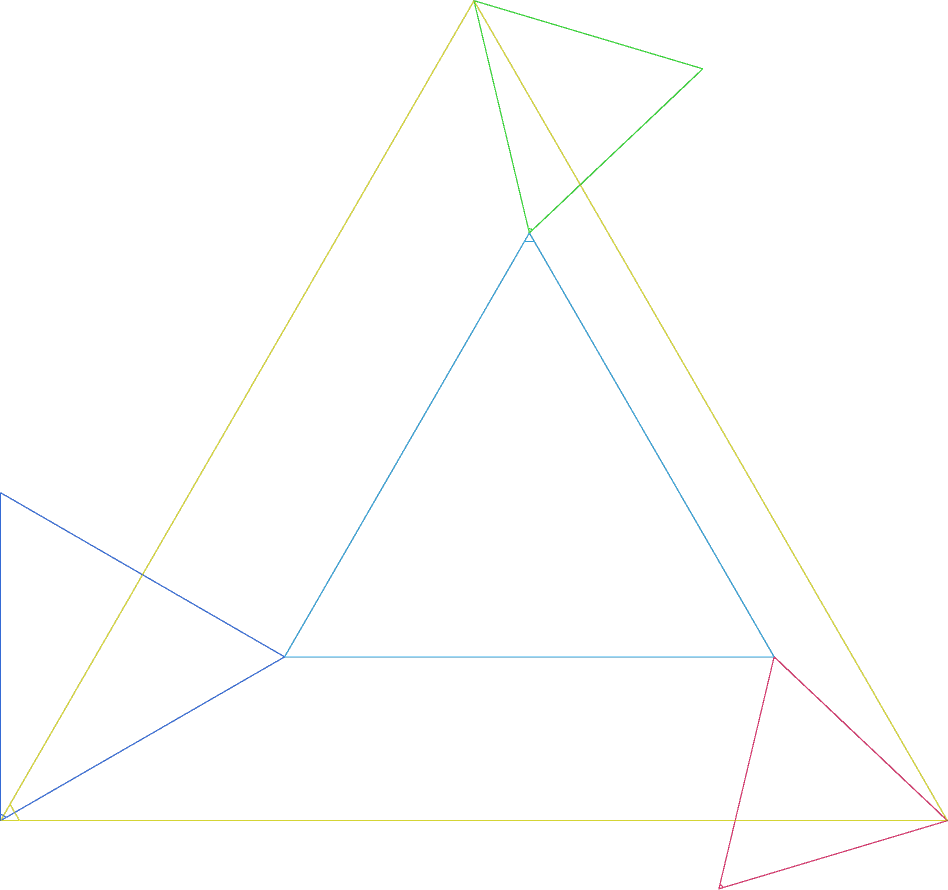
\includegraphics[width=0.45\linewidth]{261.png}
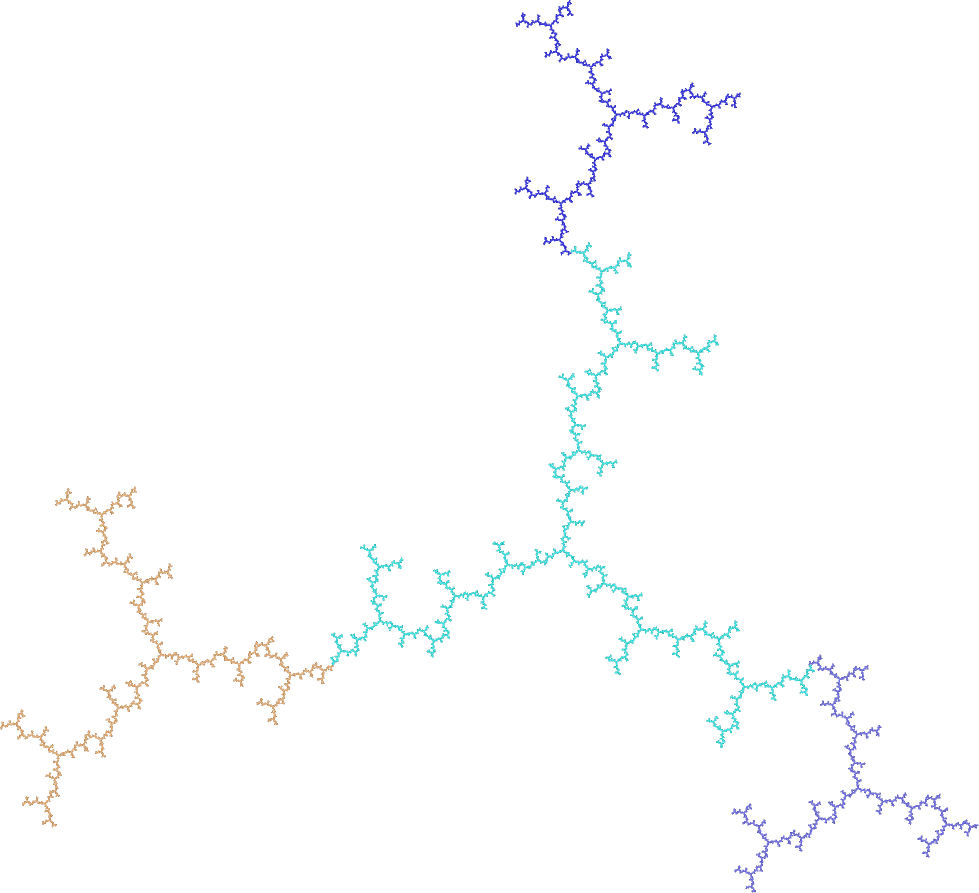
\includegraphics[width=0.45\linewidth]{262.png}
\caption{А теперь дендрит}% подпись к рисунку
\label{ris46}% метка рисунка для ссылки на него  \ref{ris46}
\end{minipage}
\end{center}
\end{figure}

На рисунках \ref{ris27}, \ref{ris28} и \ref{ris29} показана симметричная деформация. Такие полигональные системы попадают под условие{\bf (D5)}, а значит поворот подобий системы не изменит её аттрактор.

\begin{figure}[h!]
\centering
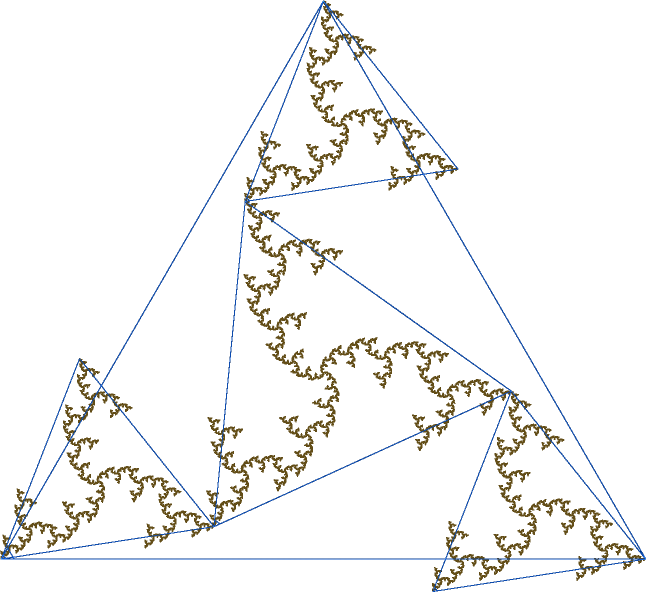
\includegraphics[width=0.75\linewidth]{2_7.png}
\caption{дендрит} % подпись к рисунку
\label{ris27} % метка рисунка для ссылки на него  \ref{ris27}
\end{figure}

\newpage
\begin{figure}[h!]
\centering
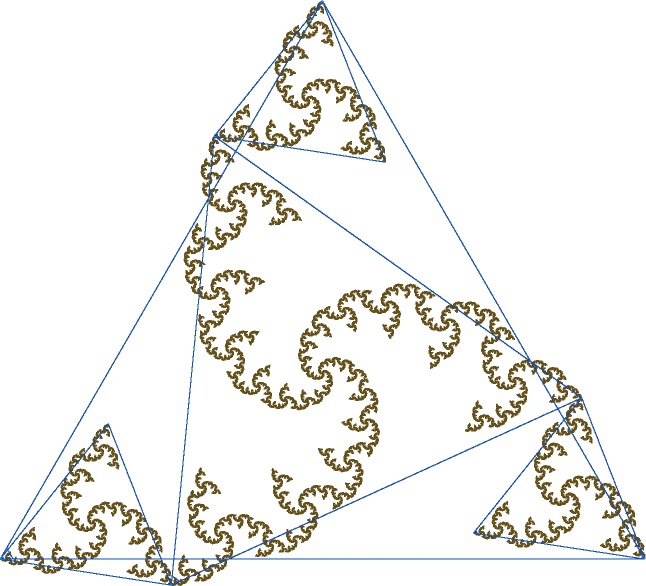
\includegraphics[width=0.69\linewidth]{2_8.png}
\caption{дендрит}% подпись к рисунку
\label{ris28}% метка рисунка для ссылки на него  \ref{ris28}
\end{figure}

\begin{figure}[h!]
\centering
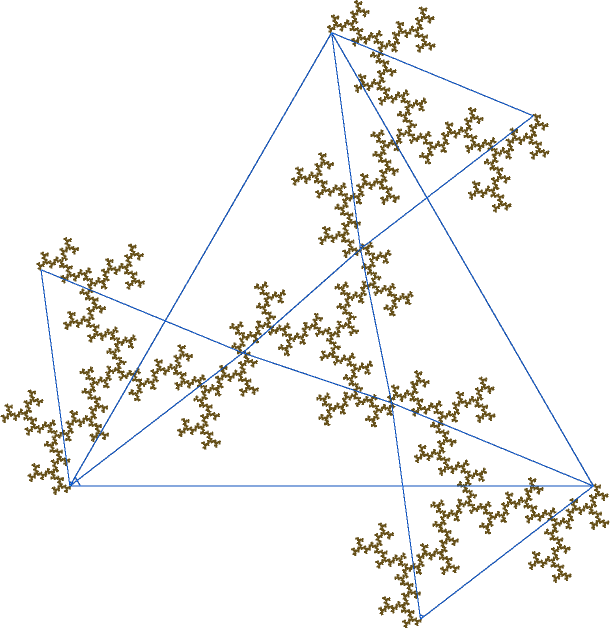
\includegraphics[width=0.69\linewidth]{2_9.png}
\caption{дендрит}% подпись к рисунку
\label{ris29}% метка рисунка для ссылки на него  \ref{ris29}
\end{figure}
\newpage

На рисунках \ref{ris210} и \ref{ris211} показан дендрит и его полигональная система. Это один из тех случаев обобщенных полигональных систем, которые не попадают под категорию деформаций.

\begin{figure}[h!]
\centering
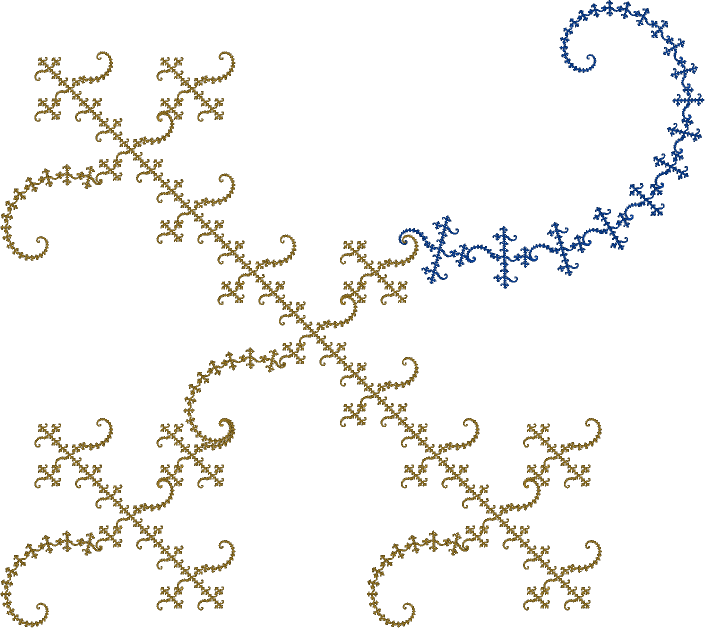
\includegraphics[width=0.68\linewidth]{2_10.png}
\caption{дендрит}% подпись к рисунку
\label{ris210}% метка рисунка для ссылки на него  \ref{ris210}
\end{figure}

\begin{figure}[h!]
\centering
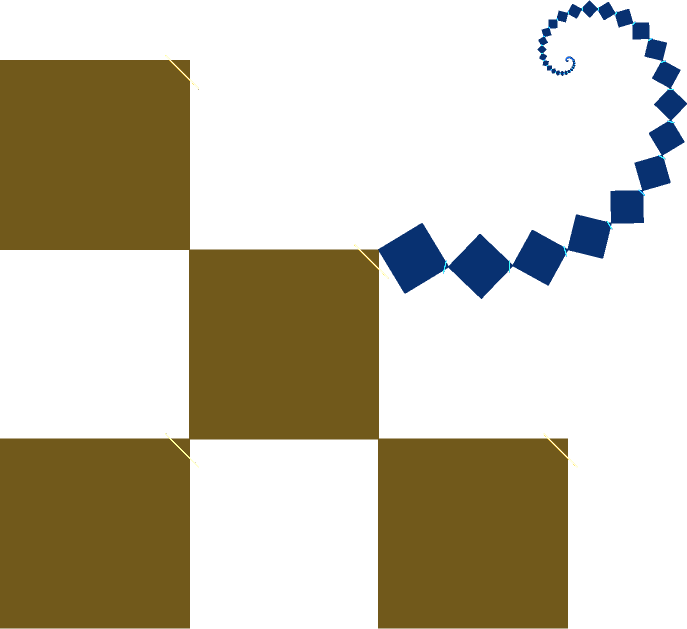
\includegraphics[width=0.68\linewidth]{2_11.png}
\caption{полигональная система}% подпись к рисунку
\label{ris211}% метка рисунка для ссылки на него  \ref{ris211}
\end{figure}

\newpage

На рисунках \ref{ris212} и \ref{ris213} показан дендрит и его полигональная система. В первом случае показана симметричная деформация, во втором для этого же дендрита представлена стягиваемая полигональная система с многоугольником из локсодром. Использование локсодромных многоугольников еще изучается.

\begin{figure}[h!]
\centering
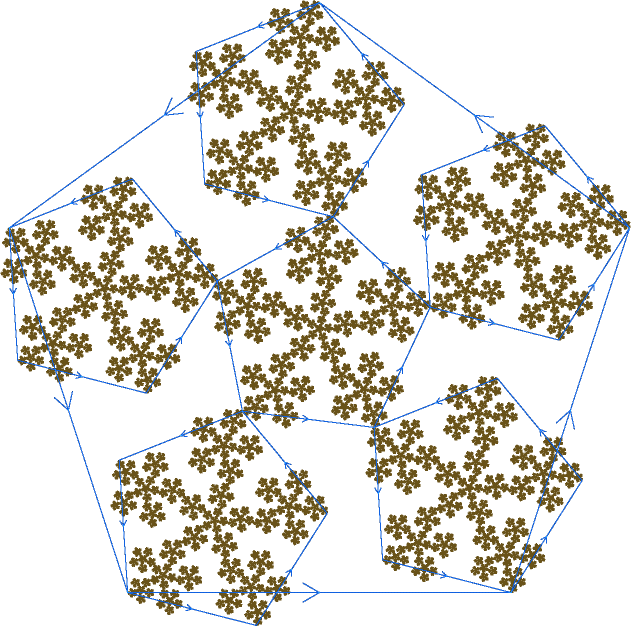
\includegraphics[width=1\linewidth]{2_12.png}
\caption{дендрит}% подпись к рисунку
\label{ris212}% метка рисунка для ссылки на него  \ref{ris212}
\end{figure}

\newpage
\begin{figure}[h!]
\centering
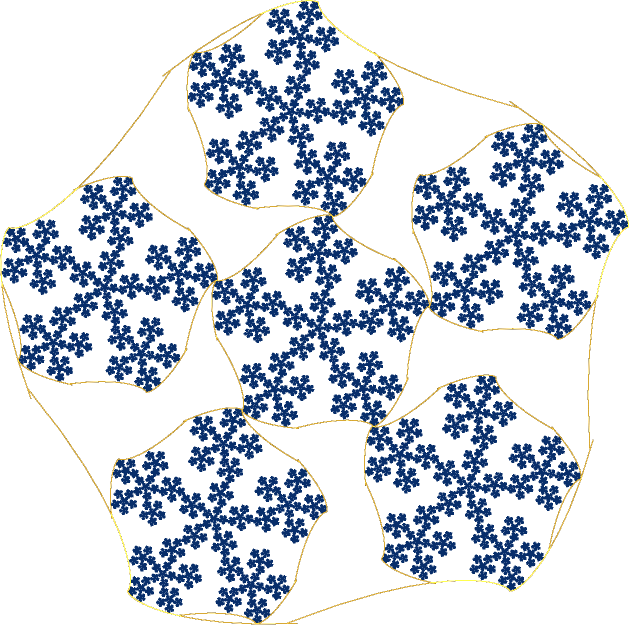
\includegraphics[width=1\linewidth]{2_13.png}
\caption{дендрит и локсодромные полиэдры}% подпись к рисунку
\label{ris213}% метка рисунка для ссылки на него  \ref{ris213}
\end{figure}

На следующем рисунке представлена деформация стягиваемой полигональной системы из рисунка \ref{ris142} из прошлого раздела:

\newpage
\begin{figure}[h!]
\centering
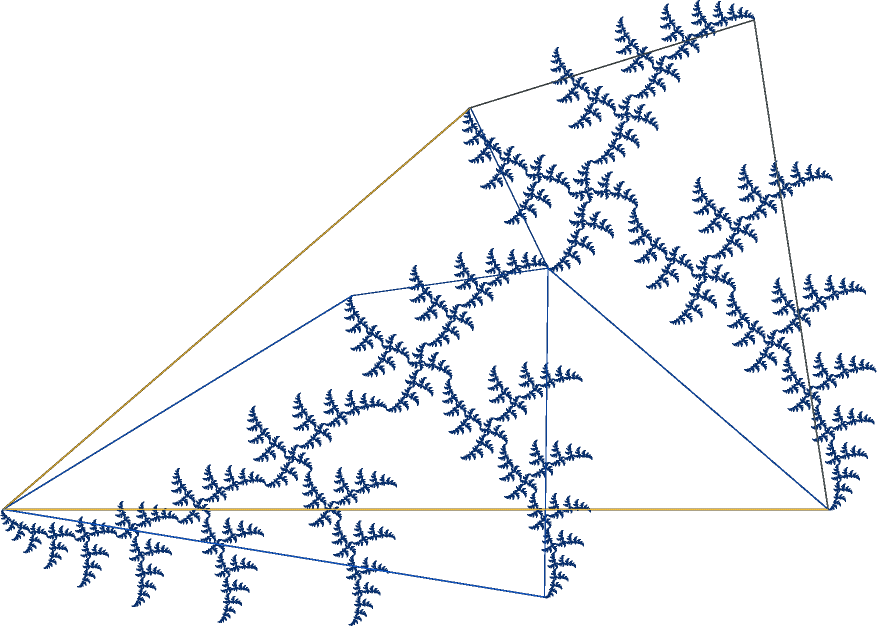
\includegraphics[width=1\linewidth]{2_14.png}
\caption{дендрит}% подпись к рисунку
\label{ris214}% метка рисунка для ссылки на него  \ref{ris214}
\end{figure}